\documentclass[usenames,dvipsnames, 18pt, compress, aspectratio=169]{beamer}

% can be compiled by xelatex -shell-escape presentation.tex
% lualatex -shell-escape presentation.tex

\usetheme[]{metropolis}

\usepackage[utf8]{inputenc}
\usepackage[russian, english]{babel}
\usepackage{booktabs}
\usepackage[scale=2]{ccicons}
\usepackage{listings}
\usepackage{marvosym}
\usepackage{color}
\usepackage{xcolor}
\usepackage[document]{ragged2e}
\usepackage[export]{adjustbox}
\usepackage{fontawesome}
\usepackage{enumitem}
\usepackage{minted}
\usemintedstyle{tango}
\usepackage[normalem]{ulem}
\usepackage{tikz}
\usetikzlibrary{patterns}
\usetikzlibrary{mindmap}
\usepackage{graphicx}
\usepackage{eso-pic}
\usepackage{verbatim}
\usepackage{smartdiagram}
\usesmartdiagramlibrary{additions}
\usetikzlibrary{trees}
\usepackage{datetime}

\usepackage{tcolorbox}
\usepackage{tabularx}
\usepackage{array}
\usepackage{colortbl}
\tcbuselibrary{skins}

\usetikzlibrary{shapes,arrows,positioning}
\graphicspath{{images/}}
\newfontfamily{\FA}{FontAwesome}

\definecolor{check}{rgb}{0.1,2,0.3}
\definecolor{fail}{rgb}{2,0.1,0.1}
\definecolor{question}{rgb}{0.9,0.9,0.0}

\def\twitter{{\FA \faTwitter}}
\def\github{{\FA \faGithub}}
\def\email{{\FA \faEnvelope}}
\def\spin{{\FA \faSpinner}}
\def\check{\textcolor{check}{\FA \faCheck}}
\def\fail{\textcolor{fail}{\FA \faRemove}}
\def\question{\textcolor{question}{\FA \faSearch}}

\renewcommand{\ttdefault}{pcr}
\newfontfamily{\ttfamily}{Fira Code}

\usefonttheme{professionalfonts} % using non standard fonts for beamer
\usefonttheme{serif} % default family is serif
\usepackage{fontspec}
\setmainfont{Liberation Sans}
\newfontfamily\ExtraLight{Liberation Sans}
\newfontfamily\Light{Liberation Sans}
\newfontfamily\Book{Liberation Sans}
\newfontfamily\Medium{Liberation Sans}

\makeatletter
\newcommand\HUGE{\@setfontsize\Huge{32}{41}}
\makeatother

\newcommand\AtPagemyUpperLeft[1]{\AtPageLowerLeft{%
\put(\LenToUnit{0.85\paperwidth},\LenToUnit{0.05\paperheight}){#1}}}

\newcommand\AtPagemyUpperTop[1]{\AtPageLowerLeft{%
\put(\LenToUnit{0.42\paperwidth},\LenToUnit{0.90\paperheight}){#1}}}

\renewcommand{\ULthickness}{2.0pt}

\definecolor{links}{HTML}{0099FF}
\hypersetup{colorlinks, linkcolor=, urlcolor=links}

\setbeamerfont{section title}{family=\Book, size=\Huge, shape=\normalfont}
\setbeamerfont{frametitle}{family=\Book, size=\large, shape=\normalfont}
\setbeamerfont{title}{family=\Book, size=\Large, shape=\normalfont}
\setbeamerfont{subtitle}{size=\small}
\setbeamerfont{author}{family=\ExtraLight, size=\footnotesize}

\definecolor{cec1d24}{RGB}{236,29,36}
\definecolor{cffffff}{RGB}{255,255,255}

\newcommand{\ucmark}{\tikz[y=0.80pt,x=0.80pt,yscale=-0.02,xscale=0.02, inner sep=0pt, outer sep=0pt]%
  {\path[fill=cec1d24,nonzero rule] (635.8833,600.0000) .. controls
    (651.0771,599.6647) and (665.7558,591.6224) .. (673.9783,577.5525) .. controls
    (682.1001,563.3625) and (681.7384,546.6500) .. (674.5074,533.1862) --
    (378.4699,21.6487) .. controls (370.6590,8.7662) and (356.3424,0.0975) ..
    (340.1099,-0.0063) .. controls (323.6499,0.0972) and (309.3362,8.7657) ..
    (301.4862,21.6487) -- (5.4612,533.1862) .. controls (-1.7257,546.6500) and
    (-2.0877,563.3625) .. (5.9903,577.5525) .. controls (14.2570,591.6225) and
    (28.9353,599.6650) .. (44.0853,600.0000) -- (635.8853,600.0000);
    \path[fill=cffffff,nonzero rule] (340.1208,75.7875) -- (71.0683,540.8450) --
    (608.8933,540.8450) -- (340.1058,75.7950);
    \path[fill=black,nonzero rule] (303.5900,225.7800) .. controls
    (280.4500,225.7300) and (276.9200,248.1400) .. (276.8800,250.6200) .. controls
    (276.9200,262.4400) and (285.4000,277.1700) .. (309.1600,279.4100) .. controls
    (309.1600,279.4100) and (313.7700,280.0900) .. (313.6600,283.0900) .. controls
    (313.7700,285.9400) and (313.7800,284.9700) .. (312.3400,286.5300) .. controls
    (310.8500,288.2300) and (298.5500,299.6400) .. (298.3100,302.6600) .. controls
    (296.9800,316.8800) and (300.1800,335.2800) .. (303.0900,345.9400) .. controls
    (303.0900,345.9400) and (306.6000,354.7800) .. (303.8800,361.0000) .. controls
    (301.0600,367.4700) and (289.0000,397.7400) .. (288.0000,399.5600) .. controls
    (285.1300,404.8200) and (284.0000,409.1400) .. (285.8800,415.4100) .. controls
    (284.6600,416.1100) and (264.4700,428.8800) .. (264.4700,428.8800) .. controls
    (264.4700,428.8800) and (261.3500,421.5100) .. (253.5900,419.3800) .. controls
    (245.7000,417.1100) and (239.1800,418.1800) .. (232.7200,405.9100) --
    (226.8800,396.4100) .. controls (226.8800,396.4100) and (225.6700,392.9300) ..
    (219.7500,391.6200) .. controls (213.9300,390.4900) and (206.1000,388.3000) ..
    (202.8100,388.4700) .. controls (198.6100,388.8800) and (195.2200,387.7300) ..
    (189.5900,394.2800) .. controls (185.0800,399.5300) and (112.8800,524.4700) ..
    (112.8800,524.4700) -- (286.4100,524.4700) .. controls (286.4100,524.4700) and
    (290.7100,524.0000) .. (289.5900,519.9700) .. controls (288.2700,516.1900) and
    (267.3800,441.8100) .. (267.3800,441.8100) -- (291.4400,426.7500) .. controls
    (291.4400,426.7500) and (293.3600,429.9900) .. (300.4400,426.7500) .. controls
    (307.3800,423.4800) and (309.9700,421.7500) .. (309.9700,421.7500) .. controls
    (309.9700,421.7500) and (313.9200,421.4900) .. (313.4100,413.0300) .. controls
    (316.1700,411.3100) and (341.9700,395.0600) .. (341.9700,395.0600) .. controls
    (341.9700,395.0600) and (332.8400,417.6000) .. (331.9100,427.5600) .. controls
    (331.2100,437.4600) and (327.6900,504.1200) .. (327.6900,504.1200) .. controls
    (327.6900,504.1200) and (328.1300,509.2200) .. (324.7800,510.2200) .. controls
    (321.2800,511.1700) and (305.7200,515.5000) .. (305.7200,515.5000) .. controls
    (305.7200,515.5000) and (301.3900,516.2100) .. (301.5000,519.7200) .. controls
    (301.3900,523.0400) and (303.0200,524.3400) .. (304.9400,524.4700) .. controls
    (306.9300,524.3400) and (355.7200,524.4700) .. (355.7200,524.4700) .. controls
    (355.7200,524.4700) and (360.7100,525.0000) .. (361.5300,518.4100) .. controls
    (362.3400,511.9900) and (371.5900,445.5000) .. (371.5900,445.5000) .. controls
    (371.5900,445.5000) and (367.5700,444.4500) .. (367.6200,440.5000) .. controls
    (367.5700,436.3200) and (367.5600,433.2000) .. (368.9400,431.5000) .. controls
    (370.1600,429.9500) and (384.8300,413.0400) .. (394.8800,389.5300) .. controls
    (396.4200,386.0300) and (397.5600,389.1300) .. (397.7800,390.0600) .. controls
    (398.2100,390.7500) and (417.2800,442.6600) .. (419.4700,444.7200) .. controls
    (421.8400,446.5600) and (473.3600,488.2300) .. (474.5000,489.0900) .. controls
    (475.6400,489.8600) and (478.9100,492.1100) .. (479.0000,499.3800) .. controls
    (478.9100,506.7600) and (475.9700,512.6300) .. (473.9700,514.9700) .. controls
    (472.0500,517.1900) and (468.8000,520.4500) .. (468.6900,521.8400) .. controls
    (468.8000,523.3800) and (470.2800,524.3400) .. (471.3400,524.4700) .. controls
    (472.5600,524.3400) and (479.2500,524.3400) .. (479.8100,524.4700) .. controls
    (480.5500,524.3400) and (489.3400,525.0100) .. (495.4100,514.1900) .. controls
    (501.7300,503.5300) and (513.1200,484.3400) .. (513.1200,484.3400) .. controls
    (513.1200,484.3400) and (515.5800,480.5600) .. (512.0600,478.2500) .. controls
    (508.4000,476.0100) and (502.7100,474.7100) .. (499.3800,471.1200) .. controls
    (495.8600,467.5500) and (462.9400,429.6400) .. (462.3400,428.8800) .. controls
    (461.9600,428.3400) and (457.7100,423.7600) .. (452.2800,426.2200) .. controls
    (450.7000,424.0900) and (448.8400,421.2200) .. (448.8400,421.2200) .. controls
    (448.8400,421.2200) and (439.4600,364.4600) .. (429.5300,340.4100) .. controls
    (431.8000,339.0000) and (434.8100,336.7200) .. (434.8100,336.7200) .. controls
    (434.8100,336.7200) and (442.7200,343.5500) .. (449.3800,336.4400) .. controls
    (456.0900,329.2300) and (455.6000,329.4100) .. (454.4100,326.1600) .. controls
    (453.3200,322.9000) and (452.8300,321.9100) .. (450.4400,320.5900) .. controls
    (448.2700,319.3000) and (444.5200,315.5500) .. (444.6200,308.9700) .. controls
    (444.5200,302.5400) and (441.7400,284.8000) .. (438.5300,277.2800) .. controls
    (435.5500,269.8300) and (434.5600,261.5500) .. (422.9100,256.4400) .. controls
    (404.4800,248.2100) and (379.8000,243.3100) .. (361.8100,247.9700) .. controls
    (356.8300,249.3000) and (340.8200,261.0500) .. (339.3100,261.9700) .. controls
    (337.8900,262.6800) and (331.6400,265.2600) .. (332.1900,259.8400) .. controls
    (333.4500,247.4700) and (322.7500,225.7300) .. (303.5900,225.7800) --
    cycle(394.8800,275.9700) .. controls (394.8800,275.9700) and
    (408.4700,275.8400) .. (411.5300,276.2200) .. controls (414.3400,276.5000) and
    (416.0300,280.1900) .. (416.0300,280.1900) -- (429.0000,325.8800) --
    (424.2500,328.7800) .. controls (421.5800,323.2700) and (397.9000,287.2600) ..
    (393.0300,280.4700) .. controls (389.9100,276.1000) and (394.8800,275.9700) ..
    (394.8800,275.9700) -- cycle(331.0000,332.8100) .. controls
    (331.5700,332.7900) and (332.2200,332.9700) .. (332.7200,333.2800) .. controls
    (337.8300,336.2000) and (347.5100,344.5400) .. (355.7200,356.0000) .. controls
    (356.7000,357.3200) and (355.7200,361.2800) .. (355.7200,361.2800) --
    (348.5900,376.0600) .. controls (348.5900,376.0600) and (317.8500,395.3700) ..
    (315.5000,396.9100) .. controls (312.9600,398.3000) and (311.5500,396.9300) ..
    (313.9400,393.7500) .. controls (327.6400,375.1200) and (332.7200,353.0000) ..
    (329.5300,335.1200) .. controls (329.2600,333.4800) and (330.0500,332.8500) ..
    (331.0000,332.8100) -- cycle;}}

\pagenumbering{gobble}

\newdateformat{specialdate}{\twodigit{\THEDAY}-\twodigit{\THEMONTH}-\THEYEAR}

\newcommand\tikzmark[1]{%
  \tikz[overlay,remember picture] \coordinate (#1);}

\setbeamertemplate{title page}
{

  \vspace*{2.1cm}
  \begin{minipage}[b][\paperheight]{\textwidth}
  \begin{center}

    \ifx\inserttitle\@empty\else
    {{% \inserttitle is nonempty
      \raggedright%
      %\linespread{1.0}%
      \usebeamerfont{title}%
      \usebeamercolor[fg]{title}%
      %\vspace*{1.3em}
      \if@noSmallCapitals%
        \inserttitle%
      \else%
        \scshape{\color{black} \textbf{\begin{center}\inserttitle\end{center}}}%
      \fi%
      \vspace*{0.3em}
    }}
    \fi

    \vspace*{0.5em}%

    \ifx\insertsubtitle\@empty\else
    {{% \insertsubtitle is nonempty
      \usebeamerfont{subtitle}%
      \usebeamercolor[fg]{subtitle}%
      {\color{black} \insertsubtitle}%
      \vspace*{3.0em}%
    }}
    \fi

    \vspace*{1.0em}%

    \usebeamerfont{author}%
    \usebeamercolor[fg]{author}%
    {\color{black} \insertauthor}%

    \vspace*{1.5em}
    \fontsize{8pt}{10}\selectfont
    {\color{black} 07-03-2019}%

    \vfill
    \vspace*{2em}
  \end{center}
  \end{minipage}
}

\setbeamertemplate{section page}
{
  \vspace{2em}
  \centering
  \begin{minipage}{22em}
    \usebeamercolor[fg]{section title}
    \usebeamerfont{section title}
    {\color{black} \insertsectionhead\\[-1ex]}
  \end{minipage}
  \par
}

\setbeamertemplate{footline}
{
\begin{beamercolorbox}[wd=\textwidth,ht=3ex,dp=3ex,leftskip=0.3cm,rightskip=0.3cm]{structure}
  \usebeamerfont{page number in head/foot}
  \insertframenumber
\end{beamercolorbox}
}

\title{POSTGRESQL\\ AT LOW LEVEL}
\subtitle{STAY CURIOUS!}
\date{\today}
\author{DMITRY DOLGOV}
\institute{}

\begin{document}
{
  \usebackgroundtemplate{
\includegraphics[width=\paperwidth]{template_2.png}}%
  \fontsize{17pt}{18}\selectfont
  \maketitle
}

\AddToShipoutPictureBG{
  \AtPagemyUpperLeft{{
\includegraphics[width=2.0cm,keepaspectratio]{logo.png}}}
}%

\setbeamertemplate{background canvas}{
\begin{tikzpicture}
    \clip (0,0) rectangle (\paperwidth,\paperheight);
    \fill[color=orange] (4cm, \paperheight-6pt) rectangle (\paperwidth-4cm,\paperheight);
\end{tikzpicture}
}

\fontsize{17pt}{18}\selectfont

\begin{frame}
    \frametitle{}
    \begin{minipage}{14cm}
        \begin{center}

        \vspace{10mm}
        
\includegraphics[width=1.0\textwidth,center]{acid_team.png}

        \vspace{5mm}

        \href{https://github.com/zalando/patroni}
             {\color{black}\normalsize{patroni}} \&
        \href{https://github.com/zalando-incubator/postgres-operator}
             {\color{black}\normalsize{postgres-operator}}
        \end{center}
    \end{minipage}
\end{frame}

%\begin{frame}
    %\frametitle{}
    %\begin{center}
    %\textbf{Plan}

        %\begin{itemize}
            %\item <+->
        %\end{itemize}

        %\begin{itemize}[]
            %\item<+-> Overview
            %\item<+-> Resources
                %\begin{itemize}[label={\MVRightarrow}]
                    %\item Execution scheduling
                    %\item Memory management
                    %\item Storage IO
                %\end{itemize}
            %\item<+-> Abstracted layers
                %\begin{itemize}[label={\MVRightarrow}]
                    %\item Virtualization
                    %\item Containerization
                %\end{itemize}
        %\end{itemize}

    %\end{center}
%\end{frame}

\fontsize{16pt}{17}\selectfont
\begin{frame}
    \frametitle{}
    \begin{center}
        \vspace{1.0cm}

        \only<1>{
            \begin{tikzpicture}
                \draw[
                    color=white
                ] (-4.75,-2.75) rectangle (4.75,2.75) node[pos=.0, label={[label distance=-5mm]45:\textbf{K8S}}] {};

                \draw[
                    line width=0.5mm,
                    rounded corners=0.2cm,
                    fill=red!30
                ] (-0.75,-0.75) rectangle (0.75,0.75) node[pos=.5] {\textbf{PG}};

                \draw[
                    line width=0.2mm,
                    rounded corners=0.2cm,
                    fill=red!30
                ] (-8.0,1.85) rectangle (-5.0,2.75) node[pos=.5] {pg\_stat\_*};

             \end{tikzpicture}
        }

        \only<2>{
            \begin{tikzpicture}
                \draw[
                    color=white
                ] (-4.75,-2.75) rectangle (4.75,2.75) node[pos=.0, label={[label distance=-5mm]45:\textbf{K8S}}] {};

                \draw[
                    line width=0.5mm,
                    rounded corners=0.2cm,
                    fill=blue!20,
                    dashed
                ] (-1.75,-1.25) rectangle (1.75,1.25) node[pos=.0, label={[label distance=-5mm]45:\textbf{OS}}] {};

                \draw[
                    line width=0.5mm,
                    rounded corners=0.2cm,
                    fill=red!30
                ] (-0.75,-0.75) rectangle (0.75,0.75) node[pos=.5] {\textbf{PG}};

                \draw[
                    line width=0.2mm,
                    rounded corners=0.2cm,
                    fill=red!30
                ] (-8.0,1.85) rectangle (-5.0,2.75) node[pos=.5] {pg\_stat\_*};

                \draw[
                    line width=0.2mm,
                    rounded corners=0.2cm,
                    fill=blue!20
                ] (-8.0,0.7) rectangle (-5.0,1.6) node[pos=.5] {CPU/IO};

             \end{tikzpicture}
        }

        \only<3>{
            \begin{tikzpicture}
                \draw[
                    color=white
                ] (-4.75,-2.75) rectangle (4.75,2.75) node[pos=.0, label={[label distance=-5mm]45:\textbf{K8S}}] {};

                \draw[
                    line width=0.5mm,
                    rounded corners=0.2cm,
                    fill=green!10,
                    dashed
                ] (-2.75,-1.75) rectangle (2.75,1.75) node[pos=.0, label={[label distance=-5mm]45:\textbf{CG}}] {};

                \draw[
                    line width=0.5mm,
                    rounded corners=0.2cm,
                    fill=blue!20,
                    dashed
                ] (-1.75,-1.25) rectangle (1.75,1.25) node[pos=.0, label={[label distance=-5mm]45:\textbf{OS}}] {};

                \draw[
                    line width=0.5mm,
                    rounded corners=0.2cm,
                    fill=red!30
                ] (-0.75,-0.75) rectangle (0.75,0.75) node[pos=.5] {\textbf{PG}};

                \draw[
                    line width=0.2mm,
                    rounded corners=0.2cm,
                    fill=red!30
                ] (-8.0,1.85) rectangle (-5.0,2.75) node[pos=.5] {pg\_stat\_*};

                \draw[
                    line width=0.2mm,
                    rounded corners=0.2cm,
                    fill=blue!20
                ] (-8.0,0.7) rectangle (-5.0,1.6) node[pos=.5] {CPU/IO};

                \draw[
                    line width=0.2mm,
                    rounded corners=0.2cm,
                    fill=green!10
                ] (-8.0,-0.45) rectangle (-5.0,0.45) node[pos=.5] {???};

             \end{tikzpicture}
        }

        \only<4>{
            \begin{tikzpicture}
                \draw[
                    color=white
                ] (-4.75,-2.75) rectangle (4.75,2.75) node[pos=.0, label={[label distance=-5mm]45:\textbf{K8S}}] {};

                \draw[
                    line width=0.5mm,
                    rounded corners=0.2cm,
                    fill=gray!10,
                    dashed
                ] (-3.75,-2.25) rectangle (3.75,2.25) node[pos=.0, label={[label distance=-5mm]45:\textbf{VM}}] {};

                \draw[
                    line width=0.5mm,
                    rounded corners=0.2cm,
                    fill=green!10,
                    dashed
                ] (-2.75,-1.75) rectangle (2.75,1.75) node[pos=.0, label={[label distance=-5mm]45:\textbf{CG}}] {};

                \draw[
                    line width=0.5mm,
                    rounded corners=0.2cm,
                    fill=blue!20,
                    dashed
                ] (-1.75,-1.25) rectangle (1.75,1.25) node[pos=.0, label={[label distance=-5mm]45:\textbf{OS}}] {};

                \draw[
                    line width=0.5mm,
                    rounded corners=0.2cm,
                    fill=red!30
                ] (-0.75,-0.75) rectangle (0.75,0.75) node[pos=.5] {\textbf{PG}};

                \draw[
                    line width=0.2mm,
                    rounded corners=0.2cm,
                    fill=red!30
                ] (-8.0,1.85) rectangle (-5.0,2.75) node[pos=.5] {pg\_stat\_*};

                \draw[
                    line width=0.2mm,
                    rounded corners=0.2cm,
                    fill=blue!20
                ] (-8.0,0.7) rectangle (-5.0,1.6) node[pos=.5] {CPU/IO};

                \draw[
                    line width=0.2mm,
                    rounded corners=0.2cm,
                    fill=green!10
                ] (-8.0,-0.45) rectangle (-5.0,0.45) node[pos=.5] {???};

                \draw[
                    line width=0.2mm,
                    rounded corners=0.2cm,
                    fill=gray!10
                ] (-8.0,-1.6) rectangle (-5.0,-0.7) node[pos=.5] {???};

            \end{tikzpicture}
        }

        \only<5>{
            \begin{tikzpicture}
                \draw[
                    line width=0.5mm,
                    rounded corners=0.2cm,
                    dashed
                ] (-4.75,-2.75) rectangle (4.75,2.75) node[pos=.0, label={[label distance=-5mm]45:\textbf{K8S}}] {};

                \draw[
                    line width=0.5mm,
                    rounded corners=0.2cm,
                    fill=gray!10,
                    dashed
                ] (-3.75,-2.25) rectangle (3.75,2.25) node[pos=.0, label={[label distance=-5mm]45:\textbf{VM}}] {};

                \draw[
                    line width=0.5mm,
                    rounded corners=0.2cm,
                    fill=green!10,
                    dashed
                ] (-2.75,-1.75) rectangle (2.75,1.75) node[pos=.0, label={[label distance=-5mm]45:\textbf{CG}}] {};

                \draw[
                    line width=0.5mm,
                    rounded corners=0.2cm,
                    fill=blue!20,
                    dashed
                ] (-1.75,-1.25) rectangle (1.75,1.25) node[pos=.0, label={[label distance=-5mm]45:\textbf{OS}}] {};

                \draw[
                    line width=0.5mm,
                    rounded corners=0.2cm,
                    fill=red!30
                ] (-0.75,-0.75) rectangle (0.75,0.75) node[pos=.5] {\textbf{PG}};

                \draw[
                    line width=0.2mm,
                    rounded corners=0.2cm,
                    fill=red!30
                ] (-8.0,1.85) rectangle (-5.0,2.75) node[pos=.5] {pg\_stat\_*};

                \draw[
                    line width=0.2mm,
                    rounded corners=0.2cm,
                    fill=blue!20
                ] (-8.0,0.7) rectangle (-5.0,1.6) node[pos=.5] {CPU/IO};

                \draw[
                    line width=0.2mm,
                    rounded corners=0.2cm,
                    fill=green!10
                ] (-8.0,-0.45) rectangle (-5.0,0.45) node[pos=.5] {???};

                \draw[
                    line width=0.2mm,
                    rounded corners=0.2cm,
                    fill=gray!10
                ] (-8.0,-1.6) rectangle (-5.0,-0.7) node[pos=.5] {???};

                \draw[
                    line width=0.2mm,
                    rounded corners=0.2cm,
                ] (-8.0,-2.75) rectangle (-5.0,-1.85) node[pos=.5] {???};

            \end{tikzpicture}
        }

    \end{center}
\end{frame}

\fontsize{17pt}{18}\selectfont

\begin{frame}
    \frametitle{}
    \begin{center}

    
\includegraphics[width=0.9\textwidth,center]{keep_your_secrets.jpg}

    \end{center}
\end{frame}

\begin{frame}
    \frametitle{}
    \begin{center}
    \textbf{Info sources}

        \begin{itemize}[]
            \item strace/GDB/Perf
            \item procfs/sysfs
            \item BPF/eBPF/BCC
        \end{itemize}

    \end{center}
\end{frame}

\begin{frame}[fragile]{}
    \frametitle{}
    \begin{center}
    \textbf{Shared memory}

        \begin{minted}[fontsize=\normalsize]{bash}
ERROR:  could not resize shared memory segment
"/PostgreSQL.699663942" to 50438144 bytes:
    No space left on device
        \end{minted}

    \end{center}
\end{frame}

\begin{frame}[fragile]{}
    \frametitle{}
    \begin{center}

        \begin{minted}[fontsize=\normalsize]{bash}
# strace -k -p PID
openat(AT_FDCWD, "/dev/shm/PostgreSQL.62223175"
ftruncate(176, 50438144)                = 0
fallocate(176, 0, 0, 50438144)          = -1 ENOSPC
 > libc-2.27.so(posix_fallocate+0x16) [0x114f76]
 > postgres(dsm_create+0x67) [0x377067]
   ...
 > postgres(ExecInitParallelPlan+0x360) [0x254a80]
 > postgres(ExecGather+0x495) [0x269115]
 > postgres(standard_ExecutorRun+0xfd) [0x25099d]
   ...
 > postgres(exec_simple_query+0x19f) [0x39afdf]
        \end{minted}

    \end{center}
\end{frame}

\begin{frame}[fragile]{}
    \frametitle{}
    \begin{center}

        \begin{minted}[fontsize=\normalsize]{bash}
            # Experiment 1
            transaction type: pg_long.sql
            latency average = 1312.903 ms

            # Experiment 2
            SQL script 1: pg_long.sql
             - weight: 1 (targets 50.0% of total)
             - latency average = 1426.928 ms

            SQL script 2: pg_short.sql
             - weight: 1 (targets 50.0% of total)
             - latency average = 303.092 ms
        \end{minted}

    \end{center}
\end{frame}
\note{
    mention that it was done on my laptop,
    say few words about pgbench setup
}

\begin{frame}
    \frametitle{}
    \begin{center}
        \textbf{Scheduling}

        \vspace{1.0cm}

        \only<1>{
            \begin{tikzpicture}
                \draw[
                    line width=0.5mm,
                    rounded corners=0.2cm,
                    dashed
                ] (0,0) rectangle (2,2) node[pos=.5] {};

                \draw[
                    line width=0.5mm,
                    rounded corners=0.2cm,
                    fill=red!30
                ] (0.25,0.25) rectangle (1.75,1.75) node[pos=.5] {\textbf{T1}};

                \draw[
                    line width=0.5mm,
                    rounded corners=0.1cm,
                    fill=red!30
                ] (2.25,0.25) rectangle (2.75,0.75) node[pos=.5] {\textbf{c}};

                \draw[
                    line width=0.5mm,
                    rounded corners=0.2cm,
                    dashed
                ] (4,0) rectangle (6,2) node[pos=.5] {};

                \draw[
                    line width=0.5mm,
                    rounded corners=0.2cm,
                    color=white
                ] (4.25,-1.25) rectangle (5.75,-2.75) node[pos=.5] {};

                \draw[
                    line width=0.5mm,
                    rounded corners=0.2cm,
                    fill=blue!30
                ] (4.25,0.25) rectangle (5.75,1.75) node[pos=.5] {\textbf{T2}};

                \draw[
                    line width=0.5mm,
                    rounded corners=0.1cm,
                    fill=blue!30
                ] (6.25,0.25) rectangle (6.75,0.75) node[pos=.5] {\textbf{c}};

            \end{tikzpicture}
        }

        \only<2>{
            \begin{tikzpicture}
                \draw[
                    line width=0.5mm,
                    rounded corners=0.2cm,
                    dashed
                ] (0,0) rectangle (2,2) node[pos=.5] {};

                \draw[
                    line width=0.5mm,
                    rounded corners=0.2cm,
                    fill=red!30
                ] (0.25,0.25) rectangle (1.75,1.75) node[pos=.5] {\textbf{T1}};

                \draw[
                    line width=0.5mm,
                    rounded corners=0.1cm,
                    fill=red!30
                ] (2.25,0.25) rectangle (2.75,0.75) node[pos=.5] {\textbf{c}};

                \draw[
                    line width=0.5mm,
                    rounded corners=0.2cm,
                    dashed
                ] (4,0) rectangle (6,2) node[pos=.5] {};

                \draw[
                    line width=0.5mm,
                    rounded corners=0.2cm,
                    fill=red!30
                ] (4.25,0.25) rectangle (5.75,1.75) node[pos=.5] {\textbf{T3}};

                \draw[
                    line width=0.5mm,
                    rounded corners=0.2cm,
                    fill=blue!30
                ] (4.25,-1.25) rectangle (5.75,-2.75) node[pos=.5] {\textbf{T2}};

                \draw[
                    line width=0.5mm,
                    rounded corners=0.1cm,
                    fill=blue!30
                ] (6.25,0.25) rectangle (6.75,0.75) node[pos=.5] {\textbf{c}};

            \end{tikzpicture}
        }

        \only<3>{
            \begin{tikzpicture}
                \draw[
                    line width=0.5mm,
                    rounded corners=0.2cm,
                    dashed
                ] (0,0) rectangle (2,2) node[pos=.5] {};

                \draw[
                    line width=0.5mm,
                    rounded corners=0.2cm,
                    fill=blue!30
                ] (0.25,0.25) rectangle (1.75,1.75) node[pos=.5] {\textbf{T2}};

                \draw[
                    line width=0.5mm,
                    rounded corners=0.1cm,
                    fill=red!30
                ] (2.25,0.25) rectangle (2.75,0.75) node[pos=.5] {\textbf{c}};

                \draw[
                    line width=0.5mm,
                    rounded corners=0.2cm,
                    dashed
                ] (4,0) rectangle (6,2) node[pos=.5] {};

                \draw[
                    line width=0.5mm,
                    rounded corners=0.2cm,
                    fill=red!30
                ] (4.25,0.25) rectangle (5.75,1.75) node[pos=.5] {\textbf{T3}};

                \draw[
                    line width=0.5mm,
                    rounded corners=0.2cm,
                    color=white
                ] (4.25,-1.25) rectangle (5.75,-2.75) node[pos=.5] {};

                \draw[
                    line width=0.5mm,
                    rounded corners=0.1cm,
                    fill=blue!30
                ] (6.25,0.25) rectangle (6.75,0.75) node[pos=.5] {\textbf{c}};

            \end{tikzpicture}
        }

        \only<4>{
            \begin{tikzpicture}
                \draw[
                    line width=0.5mm,
                    rounded corners=0.2cm,
                    dashed
                ] (0,0) rectangle (2,2) node[pos=.5] {};

                \draw[
                    line width=0.5mm,
                    rounded corners=0.2cm,
                    fill=blue!30
                ] (0.25,0.25) rectangle (1.75,1.75) node[pos=.5] {\textbf{T2}};

                \draw[
                    line width=0.5mm,
                    rounded corners=0.1cm,
                    fill=red!30
                ] (2.25,0.25) rectangle (2.75,0.75) node[pos=.5] {\textbf{c}};

                \draw[
                    <-,
                    line width=0.75mm,
                ] (2.5,0.25) to [controls=+(-90:2) and +(-90:2)]  (6.5,.5);

                \draw[
                    line width=0.5mm,
                    rounded corners=0.2cm,
                    dashed
                ] (4,0) rectangle (6,2) node[pos=.5] {};

                \draw[
                    line width=0.5mm,
                    rounded corners=0.2cm,
                    fill=red!30
                ] (4.25,0.25) rectangle (5.75,1.75) node[pos=.5] {\textbf{T3}};

                \draw[
                    line width=0.5mm,
                    rounded corners=0.2cm,
                    color=white
                ] (4.25,-1.25) rectangle (5.75,-2.75) node[pos=.5] {};

                \draw[
                    line width=0.5mm,
                    rounded corners=0.1cm,
                    fill=blue!30
                ] (6.25,0.25) rectangle (6.75,0.75) node[pos=.5] {\textbf{c}};

            \end{tikzpicture}
        }

    \end{center}
\end{frame}

\begin{frame}[fragile]{}
    \frametitle{}
    \begin{center}

        \begin{minted}[fontsize=\normalsize]{bash}
        # perf record -e cache-misses,cpu-migrations

        # Experiment 1
        12,396,382,649      cache-misses # 28.562%
         2,750              cpu-migrations

        # Experiment 2
        20,665,817,234      cache-misses # 28.533%
        10,460              cpu-migrations
        \end{minted}

    \end{center}
\end{frame}

\begin{frame}
    \frametitle{}
    \begin{center}

        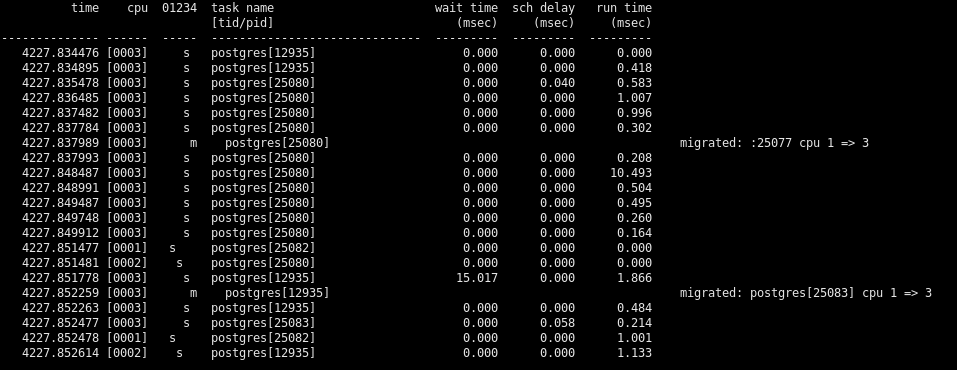
\includegraphics[width=1.0\textwidth,center]{migrations.png}

    \end{center}
\end{frame}

\begin{frame}
    \frametitle{}
    \begin{center}
    \textbf{VM}

        \begin{itemize}
            \item <+->
        \end{itemize}

        \begin{itemize}[label={\MVRightarrow}]
            \item <+-> Lock holder preemption problem
            \item <+-> Lock waiter preemption problem
            \item <+-> Intel PLE (pause loop exiting)
            \item <+-> PLE\_Gap, PLE\_Window
        \end{itemize}

        \normalsize{Intel® 64 and IA-32 Architectures Software Developer's Manual, Vol. 3}
    \end{center}
\end{frame}

\begin{frame}
    \frametitle{}
    \begin{center}
        \textbf{vCPU}

        \vspace{1.0cm}

        \only<1>{
            \begin{tikzpicture}
                \draw[
                    line width=0.5mm,
                    rounded corners=0.2cm,
                    fill=blue!30
                    ] (0,-1.25) rectangle (6.5,-2.25) node[pos=.5] {\textbf{Hypervisor}};

                \draw[
                    line width=0.5mm,
                    rounded corners=0.2cm,
                    fill=red!30
                ] (-0.5,-0.5) rectangle (1.0,1.0) node[pos=.5] {\textbf{vC1}};

                \draw[
                    line width=0.0mm,
                    color=white,
                ] (-0.5,1.0) rectangle (1.0,2.5) node[pos=.5] {};

                \draw[
                    line width=0.5mm,
                    rounded corners=0.2cm,
                    fill=red!30
                ] (1.5,-0.5) rectangle (3.0,1.0) node[pos=.5] {\textbf{vC2}};

                \draw[
                    line width=0.5mm,
                    rounded corners=0.2cm,
                    fill=gray!30
                ] (3.5,-0.5) rectangle (5.0,1.0) node[pos=.5] {\textbf{vC3}};

                \draw[
                    line width=0.5mm,
                    rounded corners=0.2cm,
                    fill=gray!30
                ] (5.5,-0.5) rectangle (7.0,1.0) node[pos=.5] {\textbf{vC4}};

            \end{tikzpicture}
        }

        \only<2>{
            \begin{tikzpicture}
                \draw[
                    line width=0.5mm,
                    rounded corners=0.2cm,
                    fill=blue!30
                    ] (0,-1.25) rectangle (6.5,-2.25) node[pos=.5] {\textbf{Hypervisor}};

                \draw[
                    line width=0.5mm,
                    rounded corners=0.2cm,
                    fill=red!30
                ] (-0.5,-0.5) rectangle (1.0,1.0) node[pos=.5] {\textbf{vC1}};

                \draw[
                    line width=0.0mm,
                    color=white,
                ] (-0.5,1.0) rectangle (1.0,2.5) node[pos=.5] {\ucmark};

                \draw[
                    line width=0.5mm,
                    rounded corners=0.2cm,
                    pattern=north west lines,
                    pattern color=red!30
                ] (1.5,-0.5) rectangle (3.0,1.0) node[pos=.5] {\textbf{vC2}};

                \draw[
                    line width=0.0mm,
                    color=white,
                ] (1.5,1.0) rectangle (3.0,2.5) node[pos=.5] {\color{black} \spin};

                \draw[
                    ->,
                    line width=0.75mm,
                ] (2.25,-0.5) to [controls=+(-135:0.8) and +(-45:0.8)]  (0.25,-0.5);

                \draw[
                    line width=0.5mm,
                    rounded corners=0.2cm,
                    fill=gray!30
                ] (3.5,-0.5) rectangle (5.0,1.0) node[pos=.5] {\textbf{vC3}};

                \draw[
                    line width=0.5mm,
                    rounded corners=0.2cm,
                    fill=gray!30
                ] (5.5,-0.5) rectangle (7.0,1.0) node[pos=.5] {\textbf{vC4}};

            \end{tikzpicture}
        }

        \only<3>{
            \begin{tikzpicture}
                \draw[
                    line width=0.5mm,
                    rounded corners=0.2cm,
                    fill=blue!30
                    ] (0,-1.25) rectangle (6.5,-2.25) node[pos=.5] {\textbf{Hypervisor}};

                \draw[
                    line width=0.5mm,
                    rounded corners=0.2cm,
                    fill=gray!30
                ] (-0.5,-0.5) rectangle (1.0,1.0) node[pos=.5] {\textbf{vC1}};

                \draw[
                    line width=0.0mm,
                    color=white,
                ] (-0.5,1.0) rectangle (1.0,2.5) node[pos=.5] {};

                \draw[
                    line width=0.5mm,
                    rounded corners=0.2cm,
                    pattern=north west lines,
                    pattern color=red!30
                ] (1.5,-0.5) rectangle (3.0,1.0) node[pos=.5] {\textbf{vC2}};

                \draw[
                    line width=0.0mm,
                    color=white,
                ] (1.5,1.0) rectangle (3.0,2.5) node[pos=.5] {\color{black} \spin};

                \draw[
                    ->,
                    line width=0.75mm,
                ] (2.25,-0.5) to [controls=+(-135:0.8) and +(-45:0.8)]  (0.25,-0.5);

                \draw[
                    line width=0.5mm,
                    rounded corners=0.2cm,
                    fill=gray!30
                ] (3.5,-0.5) rectangle (5.0,1.0) node[pos=.5] {\textbf{vC3}};

                \draw[
                    line width=0.5mm,
                    rounded corners=0.2cm,
                    fill=red!30
                ] (5.5,-0.5) rectangle (7.0,1.0) node[pos=.5] {\textbf{vC4}};

                \draw[
                    line width=0.0mm,
                    color=white,
                    ] (5.5,1.0) rectangle (7.0,2.5) node[pos=.5] {\ucmark};

            \end{tikzpicture}
        }

    \end{center}
\end{frame}

\begin{frame}[fragile]{}
    \frametitle{}
    \begin{center}

        \begin{minted}[fontsize=\normalsize]{bash}
    # latency average = 17.782 ms
    => modprobe kvm-intel ple_gap=128
    => perf record -e kvm:kvm_exit
    reason PAUSE_INSTRUCTION 306795
    
    # latency average = 16.858 ms
    => modprobe kvm-intel ple_gap=0
    => perf record -e kvm:kvm_exit
    reason PAUSE_INSTRUCTION 0
        \end{minted}

    \end{center}
\end{frame}

\begin{frame}[fragile]{}
    \frametitle{}
    \begin{center}
        \textbf{Tunables}

        \begin{flushleft}
        \begin{minted}[fontsize=\LARGE]{bash}
# from /proc/sys/kernel/
sched_wakeup_granularity_ns
# default = 1 msec * (1 + ilog(ncpus))
        \end{minted}
        \end{flushleft}

    \end{center}
\end{frame}

\begin{frame}
    \frametitle{}
    \begin{center}
		\textbf{eBPF}
        \vspace{1.0cm}

		\begin{tikzpicture}[
		  every node/.style={draw, solid, line width=0.5mm, rounded corners=0.2cm, minimum width=2cm},
          split/.style={rectangle split, rectangle split parts=2},
          to/.style={->,>=stealth',shorten >=1pt,semithick,font=\sffamily\footnotesize},
		]
			\draw node[fill=red!30] (bytecode) {Bytecode};
			\draw node[dashed, minimum width=8cm, minimum height=1cm, above=0.5cm of bytecode]
                (kernel) {Kernel};
			\draw node[split, fill=gray!30, below=0.5cm of bytecode] (stack)
                {Stack \nodepart{second} \ldots};
			\draw node[split, fill=yellow!30, left=0.5cm of stack] (regs)
                {Regs \nodepart{second} \ldots};
			\draw node[split, fill=blue!30, right=0.5cm of stack] (maps)
                {Maps \nodepart{second} \ldots};
            \draw[to] (bytecode) -- (kernel) {};
            \draw[to] (bytecode) -- (stack) {};
            \draw[to] (bytecode) -| (regs) {};
            \draw[to] (bytecode) -| (maps) {};

		 \end{tikzpicture}

    \end{center}
\end{frame}

\begin{frame}[fragile]{}
    \frametitle{}
    \begin{center}
    \textbf{pgbench and pg\_dump}

    \begin{minted}[fontsize=\scriptsize]{bash}
real    1m38.990s
user    1m9.127s
sys     0m2.066s

     usecs               : count     distribution
         0 -> 1          : 16       |                                        |
         2 -> 3          : 4604     |**                                      |
         4 -> 7          : 6812     |****                                    |
         8 -> 15         : 14888    |*********                               |
        16 -> 31         : 19267    |***********                             |
        32 -> 63         : 65795    |****************************************|
        64 -> 127        : 50454    |******************************          |
       128 -> 255        : 16393    |*********                               |
       256 -> 511        : 5981     |***                                     |
       512 -> 1023       : 12300    |*******                                 |
      1024 -> 2047       : 48       |                                        |
      2048 -> 4095       : 0        |                                        |
        \end{minted}

    \end{center}
\end{frame}

\begin{frame}[fragile]{}
    \frametitle{}
    \begin{center}
    \textbf{pgbench and pg\_dump}

    \begin{minted}[fontsize=\scriptsize]{bash}
real    1m32.030s
user    1m8.559s
sys     0m1.641s

     usecs               : count     distribution
         0 -> 1          : 1        |                                        |
         2 -> 3          : 8        |                                        |
         4 -> 7          : 25       |                                        |
         8 -> 15         : 46       |*                                       |
        16 -> 31         : 189      |*******                                 |
        32 -> 63         : 119      |****                                    |
        64 -> 127        : 96       |***                                     |
       128 -> 255        : 93       |***                                     |
       256 -> 511        : 238      |*********                               |
       512 -> 1023       : 323      |************                            |
      1024 -> 2047       : 1012     |****************************************|
      2048 -> 4095       : 47       |*                                       |
        \end{minted}

    \end{center}
\end{frame}

\begin{frame}
    \frametitle{}
    \begin{center}
    \textbf{Wakeup granularity, microsec}

        \vspace{0.5cm}
        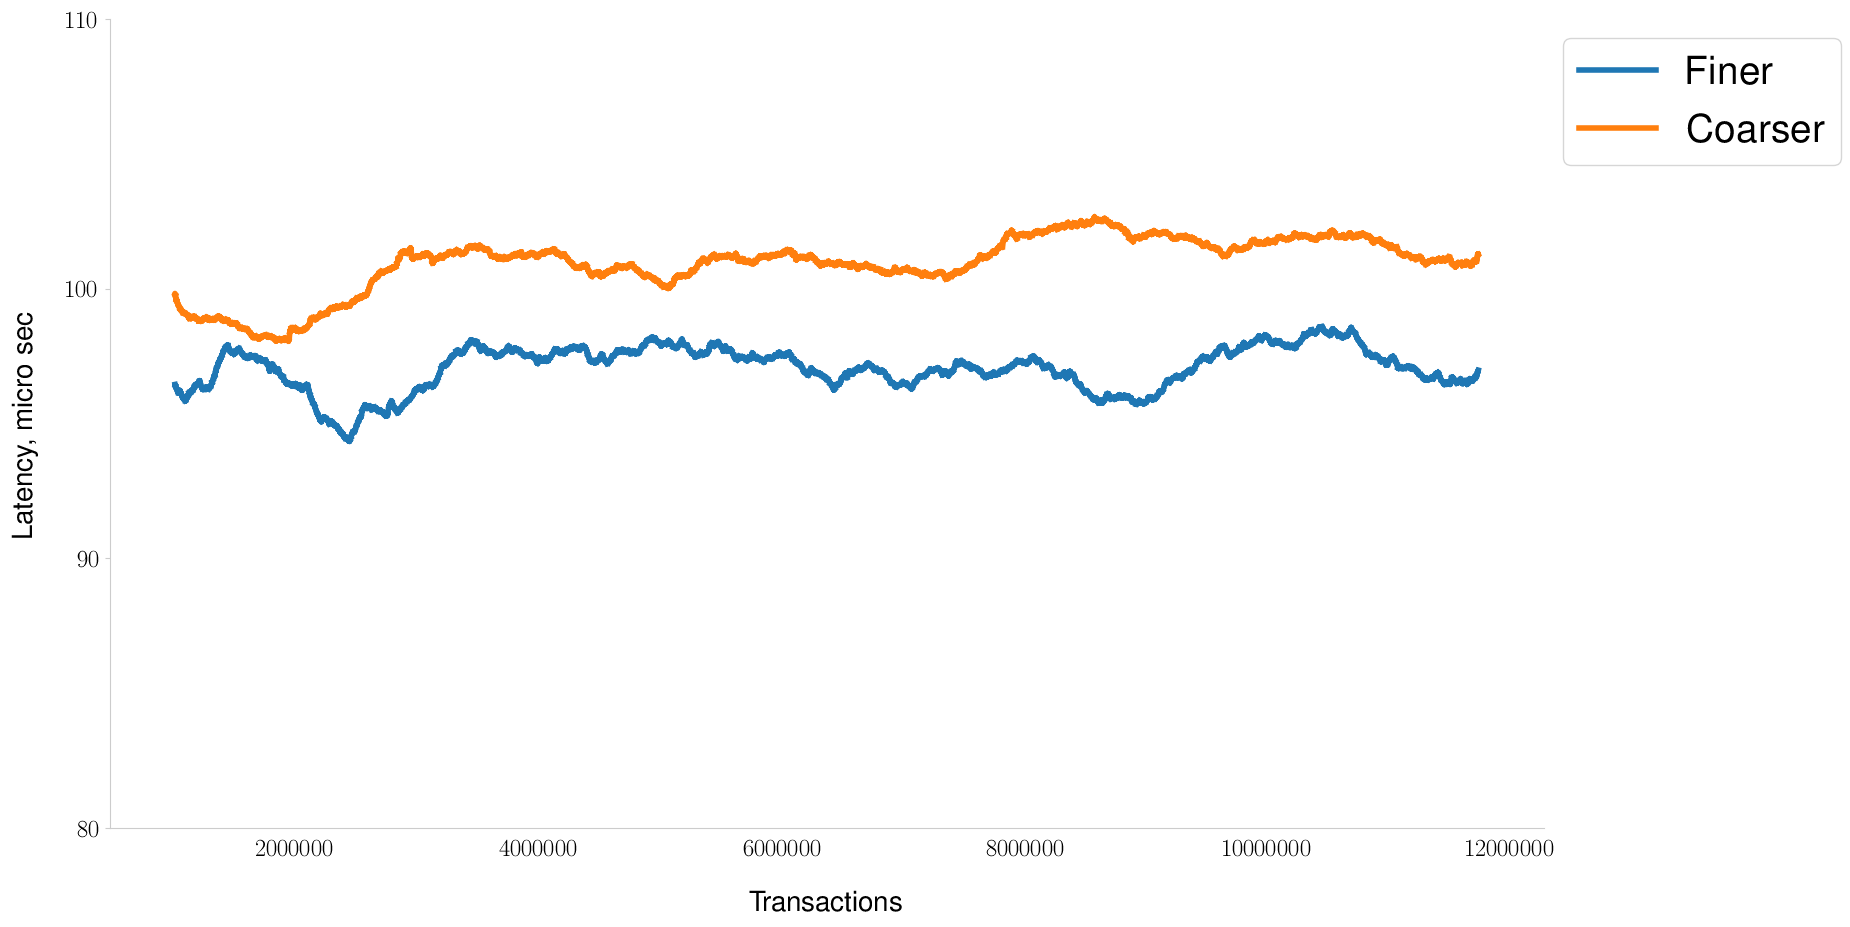
\includegraphics[width=0.9\textwidth,center]{wakeup_granularity_2.png}

    \end{center}
\end{frame}

\begin{frame}[fragile]{}
    \frametitle{}
    \begin{center}
        \textbf{Cache}

        \begin{flushleft}
		\begin{minted}[fontsize=\normalsize]{bash}
# COS1 4 cache ways, COS 2 next 8 cache ways
=> pqos -e "llc:1=0x000f;llc:2=0x0ff0;"
SOCKET 0 L3CA COS1 => MASK 0xf
SOCKET 0 L3CA COS2 => MASK 0xff0
Allocation configuration altered.
        \end{minted}
        \end{flushleft}

    \end{center}
\end{frame}

\begin{frame}
    \frametitle{}
    \begin{center}

        \begin{flushleft}
        \href{https://github.com/iovisor/bcc/}
             {\color{black}\LARGE{github.com/iovisor/bcc/}}

        \href{https://github.com/erthalion/postgres-bcc}
             {\color{black}\LARGE{github.com/erthalion/postgres-bcc}}
        \end{flushleft}

    \end{center}
\end{frame}

\begin{frame}[fragile]{}
    \frametitle{}
    \begin{center}
        \textbf{Cache}

        \begin{flushleft}
		\begin{minted}[fontsize=\normalsize]{bash}

=> llcache_per_query.py bin/postgres

PID  QUERY                      CPU REFERENCE MISS   HIT%
9720 UPDATE pgbench_tellers ... 0        2000 1000 50.00%
9720 SELECT abalance FROM   ... 2        2000  100 95.00%
...

Total References: 3303100 Total Misses: 599100 Hit Rate: 81.86%
        \end{minted}
        \end{flushleft}

    \end{center}
\end{frame}

\begin{frame}[fragile]{}
    \frametitle{}
    \begin{center}
        \textbf{Shared memory}

        \begin{flushleft}
		\begin{minted}[fontsize=\normalsize]{bash}
=> shmem.py bin/postgres

mmap:
[20439]: 142M
anon shm:
[20439]: 56B
shm:
[postmaster.opts]: 0B
[PostgreSQL.57332071]: 7K
        \end{minted}
        \end{flushleft}

    \end{center}
\end{frame}
\note{
    flashback of the first problem
}

\begin{frame}
    \frametitle{}
    \begin{center}
    \textbf{Pages written, kernel}

        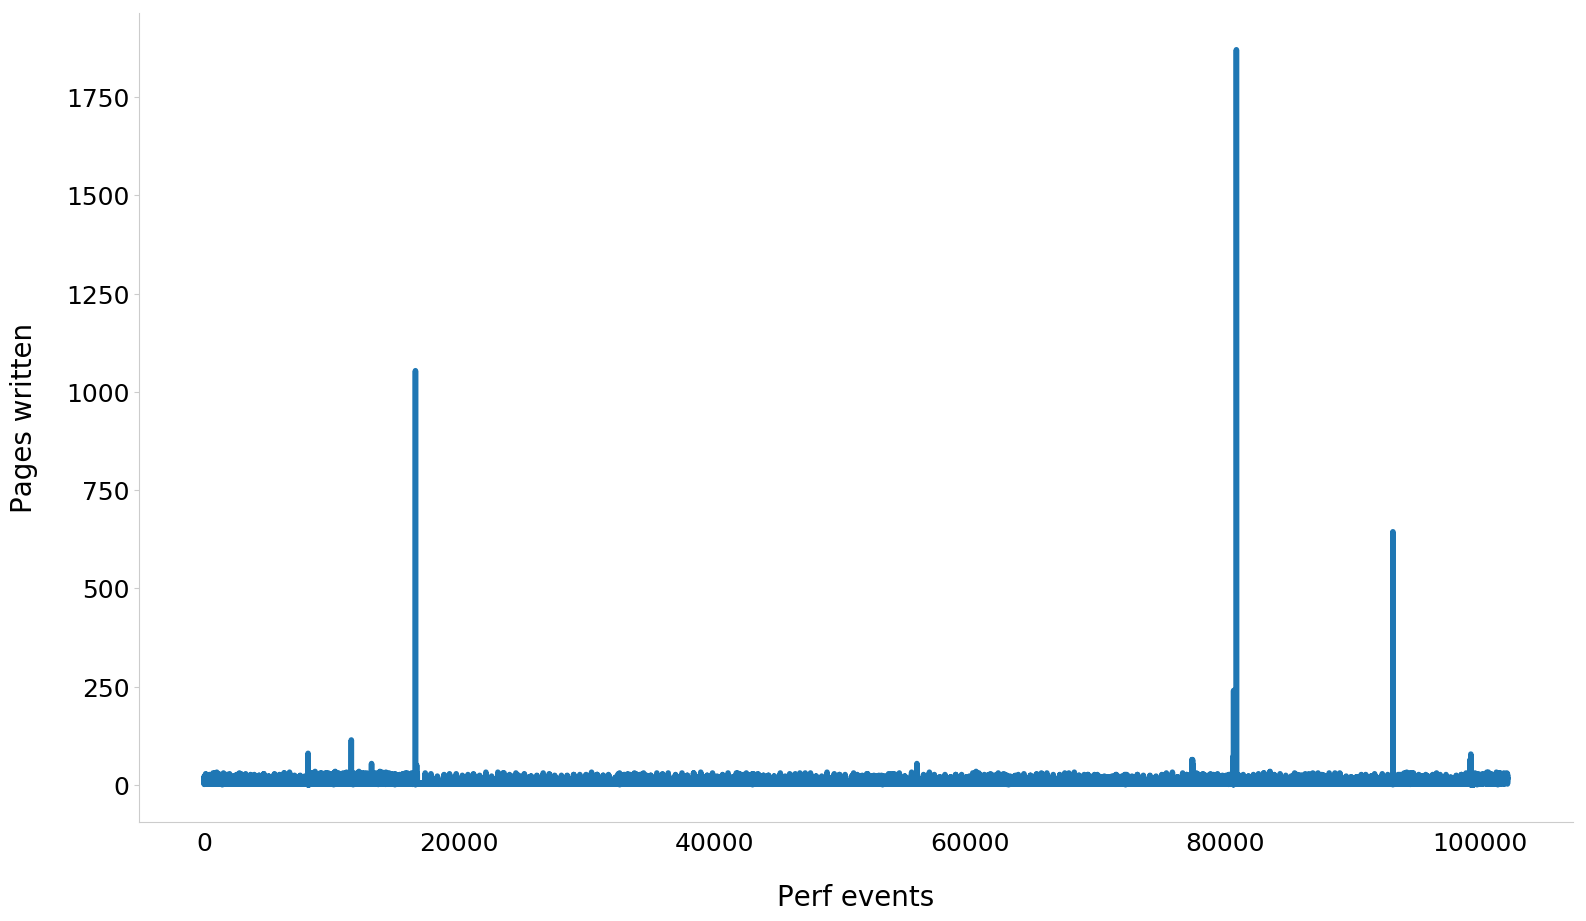
\includegraphics[width=0.84\textwidth,center]{writeback.png}

    \end{center}
\end{frame}
\note{
    pages written, but not by PostgreSQL (configured checkpoints)
}

\begin{frame}[fragile]{}
    \frametitle{}
    \begin{center}
        \textbf{Writeback (cgroup v1)}

        \begin{flushleft}
        \begin{minted}[fontsize=\normalsize]{c}
/* vmscan.c */
/* The normal page dirty throttling mechanism
 * in balance_dirty_pages() is completely broken
 * with the legacy memcg and direct stalling in
 * shrink_page_list() is used for throttling instead,
 * which lacks all the niceties such as fairness,
 * adaptive pausing, bandwidth proportional
 * allocation and configurability.
 */
static bool sane_reclaim(struct scan_control *sc)
        \end{minted}
        \end{flushleft}

    \end{center}
\end{frame}
\note{
    default hierarchy is from cgroup v2
}

\begin{frame}[fragile]{}
    \frametitle{}
    \begin{center}
        \textbf{Writeback}

        \begin{flushleft}
		\begin{minted}[fontsize=\normalsize]{bash}
=> perf record -e writeback:writeback_written

kworker/u8:1 reason=periodic   nr_pages=101429
kworker/u8:1 reason=background nr_pages=MAX_ULONG
kworker/u8:3 reason=periodic   nr_pages=101457
        \end{minted}
        \end{flushleft}

    \end{center}
\end{frame}

\begin{frame}[fragile]{}
    \frametitle{}
    \begin{center}
        \textbf{Writeback}

        \begin{flushleft}
		\begin{minted}[fontsize=\normalsize]{bash}
# pgbench insert workload
=> io_timeouts.py bin/postgres

[18335] END: MAX_SCHEDULE_TIMEOUT
[18333] END: MAX_SCHEDULE_TIMEOUT
[18331] END: MAX_SCHEDULE_TIMEOUT
[18318] truncate pgbench_history: MAX_SCHEDULE_TIMEOUT
        \end{minted}
        \end{flushleft}

    \end{center}
\end{frame}

\begin{frame}[fragile]{}
    \frametitle{}
    \begin{center}
        \textbf{Kubernetes}

\begin{columns}
\begin{column}{0.48\columnwidth}
    \begin{minted}[fontsize=\normalsize,escapeinside=??]{yaml}
resources:
  requests:
    memory: "64Mi" ?\tikzmark{memory_req}?
    cpu: "250m"
  limits:
    memory: "128Mi" ?\tikzmark{memory_lim}?
    cpu: "500m"
    \end{minted}

\end{column}

\begin{column}{0.48\columnwidth}

    \only<1>{
        \begin{tikzpicture}[remember picture,
            every node/.style={fill=red!30, rounded corners=0.2cm, minimum width=3cm},
            ]
          \draw node[] (soft_limit) {soft\_limits\_in\_bytes};
          \draw node[rounded corners=0.2cm, below=0.5cm of soft_limit] (hard_limit) {limits\_in\_bytes};

          \draw [overlay, ->, line width=3pt, red] (memory_req) -- (soft_limit.west);
          \draw [overlay, ->, line width=3pt, red] (memory_lim) -- (hard_limit.west);
        \end{tikzpicture}
    }
    \only<2>{
        \begin{tikzpicture}[remember picture,
            every node/.style={fill=red!30, rounded corners=0.2cm, minimum width=3cm},
            ]
          \draw node[] (soft_limit) {soft\_limits\_in\_bytes};
          \draw node[rounded corners=0.2cm, below=0.5cm of soft_limit] (hard_limit) {limits\_in\_bytes};

          \draw [overlay, ->, line width=3pt, red] (memory_req) -- (soft_limit.west);
          \draw [overlay, ->, line width=3pt, red] (memory_lim) -- (hard_limit.west);
        \end{tikzpicture}
    }

\end{column}
\end{columns}

    \end{center}
\end{frame}

\begin{frame}
    \frametitle{}
    \begin{center}
    \textbf{K8S}

        \begin{itemize}[]
            \item directly manageable
            \item requests $\not \to$ memory.soft\_limit\_in\_bytes
            \item limits $\to$ memory.limit\_in\_bytes (OOM)
            \item memory.kmem.limit\_in\_bytes
            \item best efforts (not everything is accounted)
        \end{itemize}

    \end{center}
\end{frame}

\begin{frame}
    \frametitle{}
    \begin{center}
    \textbf{Latency rolling standard deviation, r/w}

        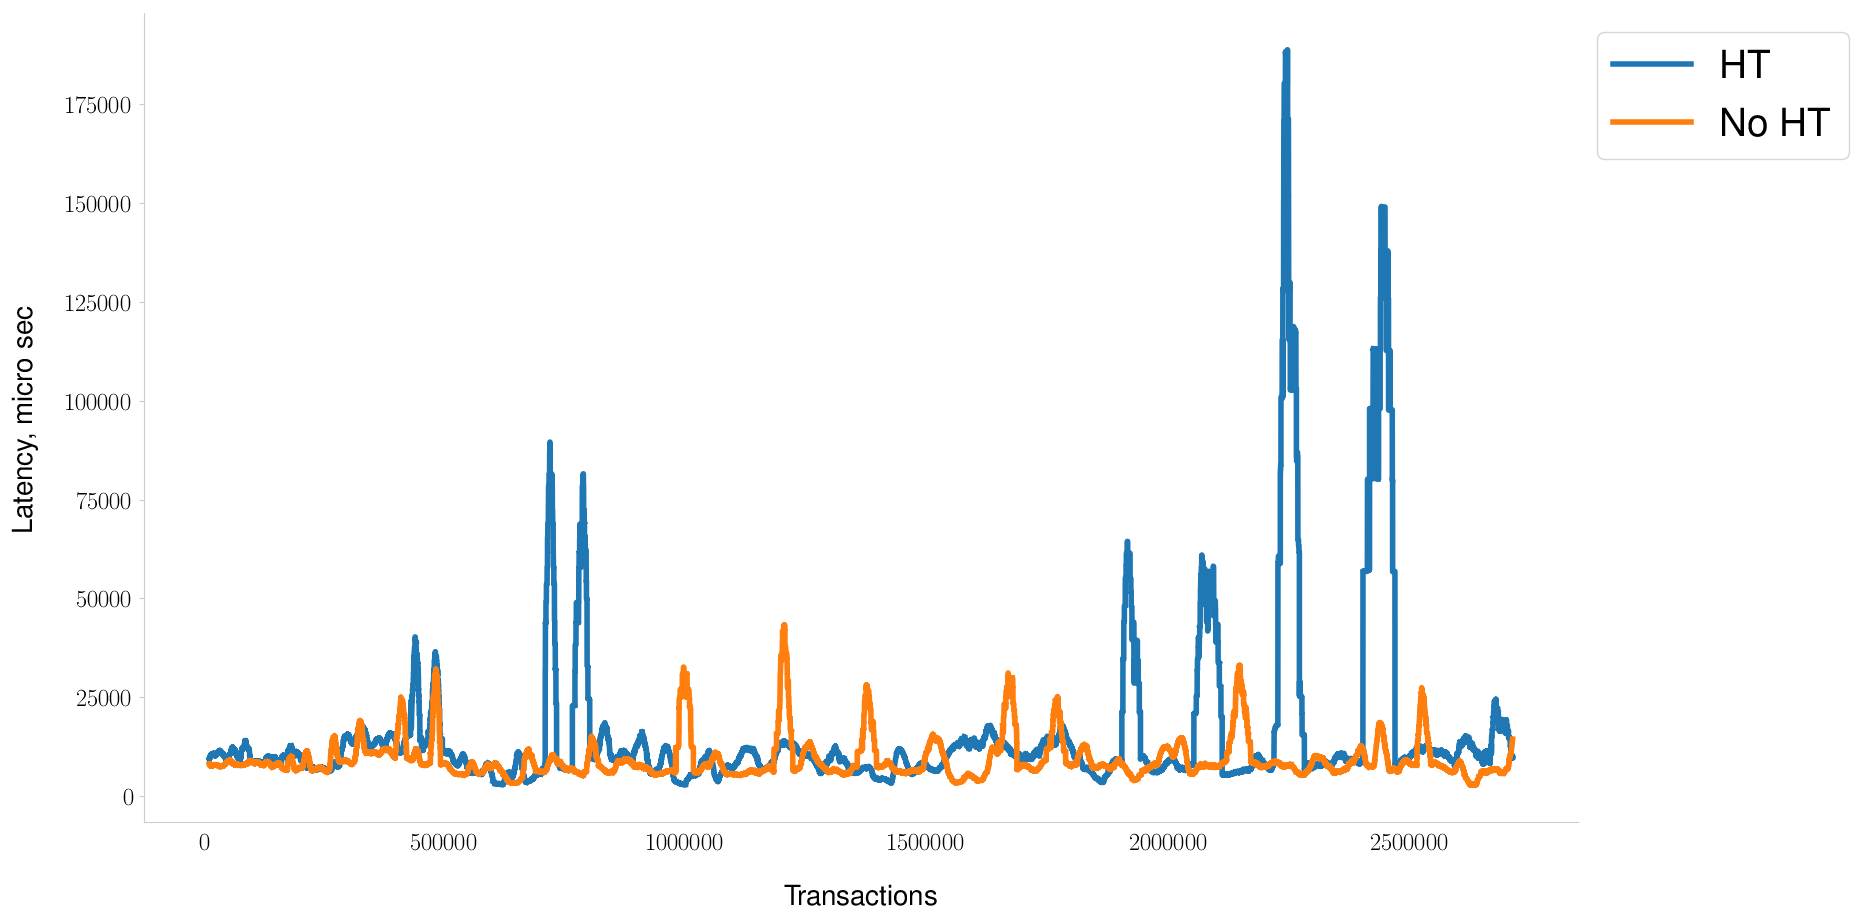
\includegraphics[width=0.9\textwidth,center]{hyperthreading_2.png}

    \end{center}
\end{frame}

\begin{frame}
    \frametitle{}
    \begin{center}
    \textbf{Latency rolling standard deviation, readonly}

        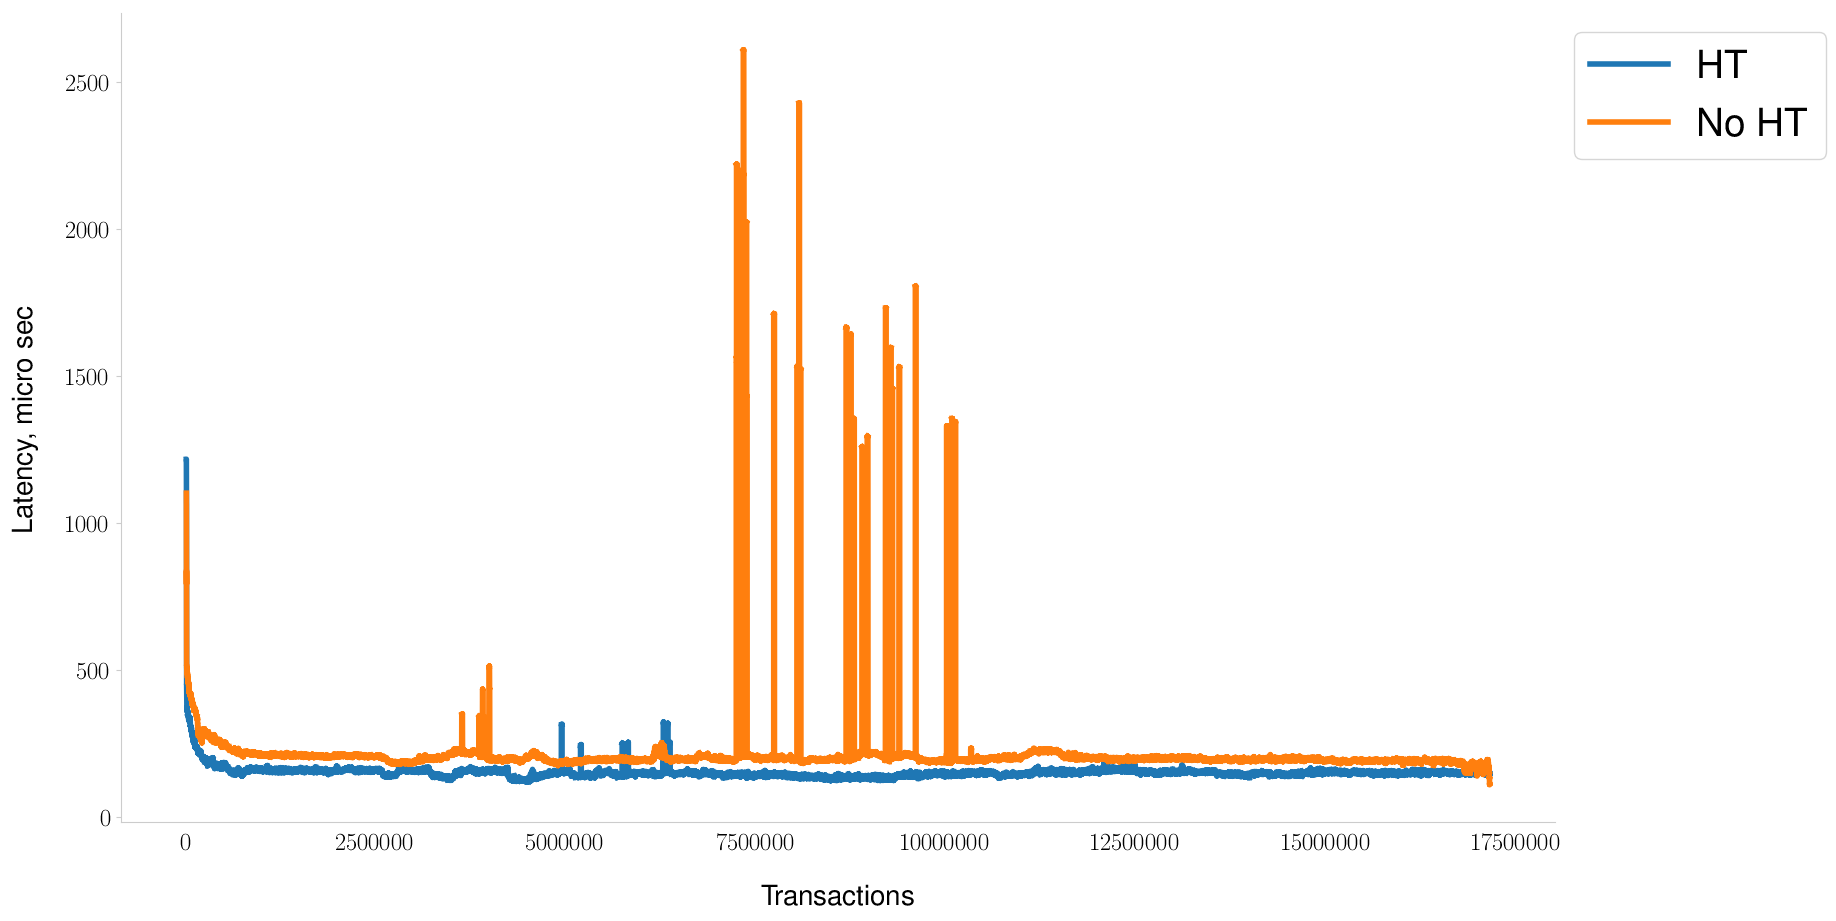
\includegraphics[width=0.9\textwidth,center]{hyperthreading_readonly_2.png}

    \end{center}
\end{frame}

\fontsize{13pt}{14}\selectfont
\section{Memory management}
\fontsize{17pt}{18}\selectfont

\begin{frame}
    \frametitle{}
    \begin{center}
        \textbf{Dirty pages}

        \vspace{1.0cm}

        \only<1>{
            \begin{tikzpicture}
                \draw[
                    line width=0.5mm,
                    rounded corners=0.2cm,
                    pattern=north west lines,
                    pattern color=blue!30
                    ] (0,-1) rectangle (6,-2) node[pos=.5] {\textbf{OS Cache}};

                \draw[
                    line width=0.5mm,
                    rounded corners=0.2cm,
                    pattern=north west lines,
                    pattern color=green!30
                    ] (0,-2.25) rectangle (6,-3.25) node[pos=.5] {\textbf{Storage}};

                \draw[
                    line width=0.5mm,
                    rounded corners=0.2cm,
                    fill=blue!30
                    ] (-3,2.75) rectangle (0,1.75) node[pos=.5] {\textbf{bgw}};

                \draw[
                    line width=0.5mm,
                    rounded corners=0.2cm,
                    color=white
                    ] (-3.1,2.85) rectangle (0.1,1.65) node[pos=.5] {};

                \draw[
                    line width=0.5mm,
                    rounded corners=0.2cm,
                    fill=blue!30
                    ] (-3,1.5) rectangle (0,0.5) node[pos=.5] {\textbf{linux}};

                \draw[
                    line width=0.5mm,
                    rounded corners=0.2cm,
                    fill=blue!30
                    ] (-3,0.25) rectangle (0,-0.75) node[pos=.5] {\textbf{chkp}};

                \draw[
                    line width=0.5mm,
                    rounded corners=0.1cm,
                    fill=red!30
                ] (1.25,2.25) rectangle (1.75,2.75) node[pos=.5] {};

                \draw[
                    line width=0.5mm,
                    rounded corners=0.1cm,
                    fill=white!30
                ] (4.25,2.25) rectangle (4.75,2.75) node[pos=.5] {};

                \draw[
                    line width=0.5mm,
                    rounded corners=0.1cm,
                    fill=white!30
                ] (3.25,2.25) rectangle (3.75,2.75) node[pos=.5] {};

                \draw[
                    line width=0.5mm,
                    rounded corners=0.1cm,
                    fill=white!30
                ] (2.25,2.25) rectangle (2.75,2.75) node[pos=.5] {};

                \draw[
                    line width=0.5mm,
                    rounded corners=0.1cm,
                    fill=white!30
                ] (1.25,1.25) rectangle (1.75,1.75) node[pos=.5] {};

                \draw[
                    line width=0.5mm,
                    rounded corners=0.1cm,
                    fill=red!30
                ] (4.25,1.25) rectangle (4.75,1.75) node[pos=.5] {};

                \draw[
                    line width=0.5mm,
                    rounded corners=0.1cm,
                    fill=white!30
                ] (3.25,1.25) rectangle (3.75,1.75) node[pos=.5] {};

                \draw[
                    line width=0.5mm,
                    rounded corners=0.1cm,
                    fill=white!30
                ] (2.25,1.25) rectangle (2.75,1.75) node[pos=.5] {};

                \draw[
                    line width=0.5mm,
                    rounded corners=0.1cm,
                    fill=white!30
                ] (1.25,0.25) rectangle (1.75,0.75) node[pos=.5] {};

                \draw[
                    line width=0.5mm,
                    rounded corners=0.1cm,
                    fill=white!30
                ] (4.25,0.25) rectangle (4.75,0.75) node[pos=.5] {};

                \draw[
                    line width=0.5mm,
                    rounded corners=0.1cm,
                    fill=red!30
                ] (3.25,0.25) rectangle (3.75,0.75) node[pos=.5] {};

                \draw[
                    line width=0.5mm,
                    rounded corners=0.1cm,
                    fill=white!30
                ] (2.25,0.25) rectangle (2.75,0.75) node[pos=.5] {};
            \end{tikzpicture}
        }

        \only<2>{
            \begin{tikzpicture}
                \draw[
                    line width=0.5mm,
                    rounded corners=0.2cm,
                    pattern=north west lines,
                    pattern color=blue!30
                    ] (0,-1) rectangle (6,-2) node[pos=.5] {\textbf{OS Cache}};

                \draw[
                    line width=0.5mm,
                    rounded corners=0.2cm,
                    pattern=north west lines,
                    pattern color=green!30
                    ] (0,-2.25) rectangle (6,-3.25) node[pos=.5] {\textbf{Storage}};

                \draw[
                    line width=0.5mm,
                    rounded corners=0.2cm,
                    fill=blue!30
                    ] (-3,2.75) rectangle (0,1.75) node[pos=.5] {\textbf{bgw}};

                \draw[
                    line width=0.5mm,
                    rounded corners=0.2cm,
                    dashed
                    ] (-3.1,2.85) rectangle (0.1,1.65) node[pos=.5] {};

                \draw[
                    line width=0.5mm,
                    rounded corners=0.2cm,
                    fill=blue!30
                    ] (-3,1.5) rectangle (0,0.5) node[pos=.5] {\textbf{linux}};

                \draw[
                    line width=0.5mm,
                    rounded corners=0.2cm,
                    fill=blue!30
                    ] (-3,0.25) rectangle (0,-0.75) node[pos=.5] {\textbf{chkp}};

                \draw[
                    line width=0.5mm,
                    rounded corners=0.1cm,
                    fill=red!30
                ] (1.25,2.25) rectangle (1.75,2.75) node[pos=.5] {};

                \draw[
                    line width=0.5mm,
                    rounded corners=0.1cm,
                    fill=white!30
                ] (4.25,2.25) rectangle (4.75,2.75) node[pos=.5] {};

                \draw[
                    line width=0.5mm,
                    rounded corners=0.1cm,
                    fill=white!30
                ] (3.25,2.25) rectangle (3.75,2.75) node[pos=.5] {};

                \draw[
                    line width=0.5mm,
                    rounded corners=0.1cm,
                    fill=white!30
                ] (2.25,2.25) rectangle (2.75,2.75) node[pos=.5] {};

                \draw[
                    line width=0.5mm,
                    rounded corners=0.1cm,
                    fill=white!30
                ] (1.25,1.25) rectangle (1.75,1.75) node[pos=.5] {};

                \draw[
                    line width=0.5mm,
                    rounded corners=0.1cm,
                    fill=red!30
                ] (4.25,1.25) rectangle (4.75,1.75) node[pos=.5] {};

                \draw[
                    line width=0.5mm,
                    rounded corners=0.1cm,
                    fill=white!30
                ] (3.25,1.25) rectangle (3.75,1.75) node[pos=.5] {};

                \draw[
                    line width=0.5mm,
                    rounded corners=0.1cm,
                    fill=white!30
                ] (2.25,1.25) rectangle (2.75,1.75) node[pos=.5] {};

                \draw[
                    line width=0.5mm,
                    rounded corners=0.1cm,
                    fill=white!30
                ] (1.25,0.25) rectangle (1.75,0.75) node[pos=.5] {};

                \draw[
                    line width=0.5mm,
                    rounded corners=0.1cm,
                    fill=white!30
                ] (4.25,0.25) rectangle (4.75,0.75) node[pos=.5] {};

                \draw[
                    line width=0.5mm,
                    rounded corners=0.1cm,
                    fill=white!30
                ] (3.25,0.25) rectangle (3.75,0.75) node[pos=.5] {};

                \draw[
                    line width=0.5mm,
                    rounded corners=0.1cm,
                    fill=white!30
                ] (2.25,0.25) rectangle (2.75,0.75) node[pos=.5] {};

                \draw[
                    line width=0.5mm,
                    rounded corners=0.1cm,
                    fill=red!30
                ] (3.25,-1.25) rectangle (3.75,-1.75) node[pos=.5] {};

                \draw[
                    ->,
                    line width=0.75mm,
                ] (3.5,0.25) to (3.5,-1.25);

             \end{tikzpicture}
        }

        \only<3>{
            \begin{tikzpicture}
                \draw[
                    line width=0.5mm,
                    rounded corners=0.2cm,
                    pattern=north west lines,
                    pattern color=blue!30
                    ] (0,-1) rectangle (6,-2) node[pos=.5] {\textbf{OS Cache}};

                \draw[
                    line width=0.5mm,
                    rounded corners=0.2cm,
                    pattern=north west lines,
                    pattern color=green!30
                    ] (0,-2.25) rectangle (6,-3.25) node[pos=.5] {\textbf{Storage}};

                \draw[
                    line width=0.5mm,
                    rounded corners=0.2cm,
                    fill=blue!30
                    ] (-3,2.75) rectangle (0,1.75) node[pos=.5] {\textbf{bgw}};

                \draw[
                    line width=0.5mm,
                    rounded corners=0.2cm,
                    color=white
                    ] (-3.1,2.85) rectangle (0.1,1.65) node[pos=.5] {};

                \draw[
                    line width=0.5mm,
                    rounded corners=0.2cm,
                    fill=blue!30
                    ] (-3,1.5) rectangle (0,0.5) node[pos=.5] {\textbf{linux}};

                \draw[
                    line width=0.5mm,
                    rounded corners=0.2cm,
                    dashed
                    ] (-3.1,1.6) rectangle (0.1,0.4) node[pos=.5] {};

                \draw[
                    line width=0.5mm,
                    rounded corners=0.2cm,
                    fill=blue!30
                    ] (-3,0.25) rectangle (0,-0.75) node[pos=.5] {\textbf{chkp}};

                \draw[
                    line width=0.5mm,
                    rounded corners=0.1cm,
                    fill=red!30
                ] (1.25,2.25) rectangle (1.75,2.75) node[pos=.5] {};

                \draw[
                    line width=0.5mm,
                    rounded corners=0.1cm,
                    fill=white!30
                ] (4.25,2.25) rectangle (4.75,2.75) node[pos=.5] {};

                \draw[
                    line width=0.5mm,
                    rounded corners=0.1cm,
                    fill=white!30
                ] (3.25,2.25) rectangle (3.75,2.75) node[pos=.5] {};

                \draw[
                    line width=0.5mm,
                    rounded corners=0.1cm,
                    fill=white!30
                ] (2.25,2.25) rectangle (2.75,2.75) node[pos=.5] {};

                \draw[
                    line width=0.5mm,
                    rounded corners=0.1cm,
                    fill=white!30
                ] (1.25,1.25) rectangle (1.75,1.75) node[pos=.5] {};

                \draw[
                    line width=0.5mm,
                    rounded corners=0.1cm,
                    fill=red!30
                ] (4.25,1.25) rectangle (4.75,1.75) node[pos=.5] {};

                \draw[
                    line width=0.5mm,
                    rounded corners=0.1cm,
                    fill=white!30
                ] (3.25,1.25) rectangle (3.75,1.75) node[pos=.5] {};

                \draw[
                    line width=0.5mm,
                    rounded corners=0.1cm,
                    fill=white!30
                ] (2.25,1.25) rectangle (2.75,1.75) node[pos=.5] {};

                \draw[
                    line width=0.5mm,
                    rounded corners=0.1cm,
                    fill=white!30
                ] (1.25,0.25) rectangle (1.75,0.75) node[pos=.5] {};

                \draw[
                    line width=0.5mm,
                    rounded corners=0.1cm,
                    fill=white!30
                ] (4.25,0.25) rectangle (4.75,0.75) node[pos=.5] {};

                \draw[
                    line width=0.5mm,
                    rounded corners=0.1cm,
                    fill=white!30
                ] (3.25,0.25) rectangle (3.75,0.75) node[pos=.5] {};

                \draw[
                    line width=0.5mm,
                    rounded corners=0.1cm,
                    fill=white!30
                ] (2.25,0.25) rectangle (2.75,0.75) node[pos=.5] {};

                \draw[
                    line width=0.5mm,
                    rounded corners=0.1cm,
                    fill=white!30
                ] (3.25,-1.25) rectangle (3.75,-1.75) node[pos=.5] {};

                \draw[
                    line width=0.5mm,
                    rounded corners=0.1cm,
                    fill=red!30
                ] (3.25,-2.5) rectangle (3.75,-3) node[pos=.5] {};

                \draw[
                    ->,
                    line width=0.75mm,
                ] (3.5,-1.75) to (3.5,-2.5);

            \end{tikzpicture}
        }

        \only<4>{
            \begin{tikzpicture}
                \draw[
                    line width=0.5mm,
                    rounded corners=0.2cm,
                    pattern=north west lines,
                    pattern color=blue!30
                    ] (0,-1) rectangle (6,-2) node[pos=.5] {\textbf{OS Cache}};

                \draw[
                    line width=0.5mm,
                    rounded corners=0.2cm,
                    pattern=north west lines,
                    pattern color=green!30
                    ] (0,-2.25) rectangle (6,-3.25) node[pos=.5] {\textbf{Storage}};

                \draw[
                    line width=0.5mm,
                    rounded corners=0.2cm,
                    fill=blue!30
                    ] (-3,2.75) rectangle (0,1.75) node[pos=.5] {\textbf{bgw}};

                \draw[
                    line width=0.5mm,
                    rounded corners=0.2cm,
                    color=white
                    ] (-3.1,2.85) rectangle (0.1,1.65) node[pos=.5] {};

                \draw[
                    line width=0.5mm,
                    rounded corners=0.2cm,
                    fill=blue!30
                    ] (-3,1.5) rectangle (0,0.5) node[pos=.5] {\textbf{linux}};

                \draw[
                    line width=0.5mm,
                    rounded corners=0.2cm,
                    fill=blue!30
                    ] (-3,0.25) rectangle (0,-0.75) node[pos=.5] {\textbf{chkp}};

                \draw[
                    line width=0.5mm,
                    rounded corners=0.2cm,
                    dashed
                    ] (-3.1,0.35) rectangle (0.1,-0.85) node[pos=.5] {};

                \draw[
                    line width=0.5mm,
                    rounded corners=0.1cm,
                    fill=white!30
                ] (1.25,2.25) rectangle (1.75,2.75) node[pos=.5] {};

                \draw[
                    line width=0.5mm,
                    rounded corners=0.1cm,
                    fill=white!30
                ] (4.25,2.25) rectangle (4.75,2.75) node[pos=.5] {};

                \draw[
                    line width=0.5mm,
                    rounded corners=0.1cm,
                    fill=white!30
                ] (3.25,2.25) rectangle (3.75,2.75) node[pos=.5] {};

                \draw[
                    line width=0.5mm,
                    rounded corners=0.1cm,
                    fill=white!30
                ] (2.25,2.25) rectangle (2.75,2.75) node[pos=.5] {};

                \draw[
                    line width=0.5mm,
                    rounded corners=0.1cm,
                    fill=white!30
                ] (1.25,1.25) rectangle (1.75,1.75) node[pos=.5] {};

                \draw[
                    line width=0.5mm,
                    rounded corners=0.1cm,
                    fill=white!30
                ] (4.25,1.25) rectangle (4.75,1.75) node[pos=.5] {};

                \draw[
                    line width=0.5mm,
                    rounded corners=0.1cm,
                    fill=white!30
                ] (3.25,1.25) rectangle (3.75,1.75) node[pos=.5] {};

                \draw[
                    line width=0.5mm,
                    rounded corners=0.1cm,
                    fill=white!30
                ] (2.25,1.25) rectangle (2.75,1.75) node[pos=.5] {};

                \draw[
                    line width=0.5mm,
                    rounded corners=0.1cm,
                    fill=white!30
                ] (1.25,0.25) rectangle (1.75,0.75) node[pos=.5] {};

                \draw[
                    line width=0.5mm,
                    rounded corners=0.1cm,
                    fill=white!30
                ] (4.25,0.25) rectangle (4.75,0.75) node[pos=.5] {};

                \draw[
                    line width=0.5mm,
                    rounded corners=0.1cm,
                    fill=white!30
                ] (3.25,0.25) rectangle (3.75,0.75) node[pos=.5] {};

                \draw[
                    line width=0.5mm,
                    rounded corners=0.1cm,
                    fill=white!30
                ] (2.25,0.25) rectangle (2.75,0.75) node[pos=.5] {};

                \draw[
                    line width=0.5mm,
                    rounded corners=0.1cm,
                    fill=white!30
                ] (4.25,-1.25) rectangle (4.75,-1.75) node[pos=.5] {};

                \draw[
                    line width=0.5mm,
                    rounded corners=0.1cm,
                    fill=red!30
                ] (4.25,-2.5) rectangle (4.75,-3) node[pos=.5] {};

                \draw[
                    line width=0.5mm,
                    rounded corners=0.1cm,
                    fill=white!30
                ] (1.25,-1.25) rectangle (1.75,-1.75) node[pos=.5] {};

                \draw[
                    line width=0.5mm,
                    rounded corners=0.1cm,
                    fill=red!30
                ] (1.25,-2.5) rectangle (1.75,-3) node[pos=.5] {};

                \draw[
                    line width=0.5mm,
                    rounded corners=0.1cm,
                    fill=white!30
                ] (3.25,-1.25) rectangle (3.75,-1.75) node[pos=.5] {};

                \draw[
                    line width=0.5mm,
                    rounded corners=0.1cm,
                    fill=red!30
                ] (3.25,-2.5) rectangle (3.75,-3) node[pos=.5] {};

                \draw[
                    ->,
                    line width=0.75mm,
                ] (1.5,2.25) to (1.5,-1.25);

                \draw[
                    ->,
                    line width=0.75mm,
                ] (4.5,2.25) to (4.5,-1.25);

                \draw[
                    ->,
                    line width=0.75mm,
                ] (1.5,-1.75) to (1.5,-2.5);

                \draw[
                    ->,
                    line width=0.75mm,
                ] (4.5,-1.75) to (4.5,-2.5);

            \end{tikzpicture}
        }

    \end{center}
\end{frame}

\begin{frame}
    \frametitle{}
    \begin{center}
    \textbf{Dirty pages, r/w}

        \begin{itemize}[label={\MVRightarrow}]
            \item vm.dirty\_ratio               20
            \item vm.dirty\_background\_ratio   10
            \item vm.dirty\_bytes               0
            \item vm.dirty\_backround\_bytes    0
        \end{itemize}

    \end{center}
\end{frame}

\begin{frame}
    \frametitle{}
    \begin{center}
    \textbf{Dirty pages}

    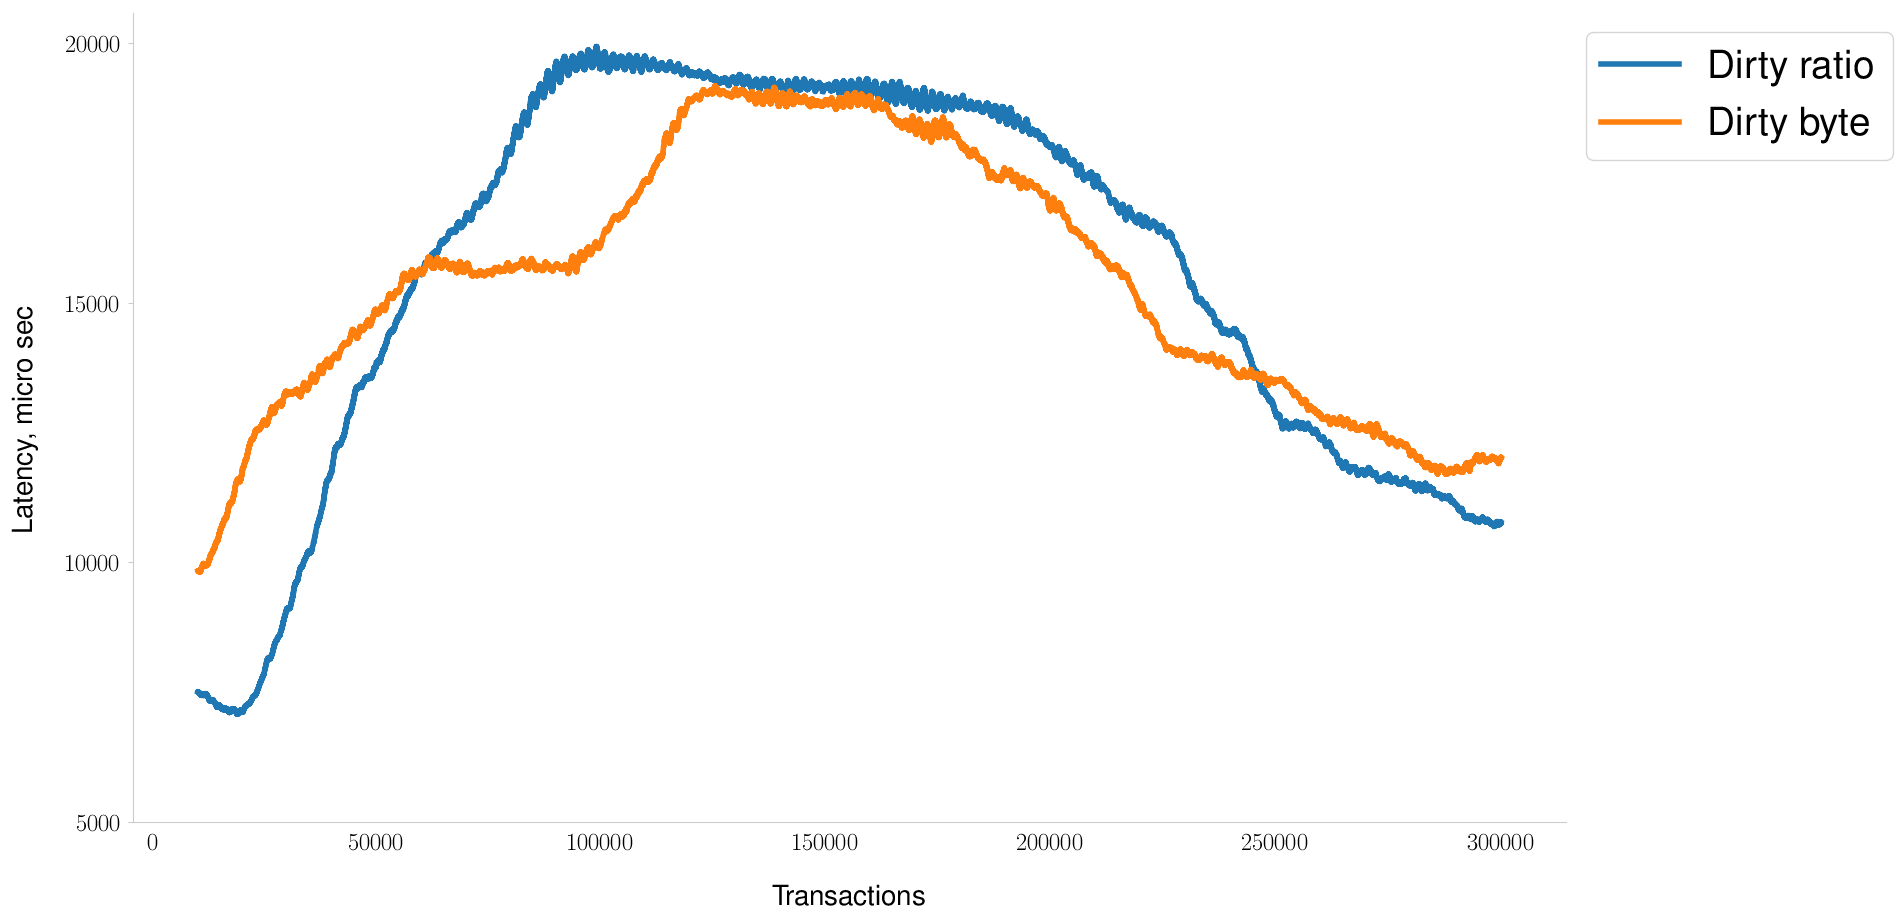
\includegraphics[width=0.9\textwidth,center]{checkpoint_dirty_pages_2.png}

    \end{center}
\end{frame}

\fontsize{13pt}{14}\selectfont
\section{Storage IO}
\fontsize{17pt}{18}\selectfont

\begin{frame}
    \frametitle{}
    \begin{center}
        \textbf{WAL}

        \vspace{1.0cm}

        \only<1>{
            \begin{tikzpicture}
                \draw[
                    -,
                    line width=0.75mm,
                    dashed
                ] (-1,-2.5) to (9,-2.5);

                \draw[
                    line width=0.5mm,
                    rounded corners=0.2cm,
                    pattern=north west lines,
                    pattern color=green!30
                    ] (-1,-3) rectangle (9,-4) node[pos=.5] {\textbf{storage}};

                \draw[
                    line width=0.5mm,
                    rounded corners=0.2cm,
                    fill=blue!30
                    ] (0,0) rectangle (2,1) node[pos=.5] {\textbf{client}};

                \draw[
                    line width=0.5mm,
                    rounded corners=0.2cm,
                    color=white
                    ] (3,0) rectangle (5,1) node[pos=.5] {};

                \draw[
                    line width=0.5mm,
                    rounded corners=0.2cm,
                    color=white
                    ] (6,0) rectangle (8,1) node[pos=.5] {};

                \draw[
                    line width=0.5mm,
                    rounded corners=0.2cm,
                    color=white
                    ] (0.5,-1) rectangle (1.5,-2) node[pos=.5] {};

            \end{tikzpicture}
        }

        \only<2>{
            \begin{tikzpicture}
                \draw[
                    -,
                    line width=0.75mm,
                    dashed
                ] (-1,-2.5) to (9,-2.5);

                \draw[
                    line width=0.5mm,
                    rounded corners=0.2cm,
                    pattern=north west lines,
                    pattern color=green!30
                    ] (-1,-3) rectangle (9,-4) node[pos=.5] {\textbf{storage}};

                \draw[
                    line width=0.5mm,
                    rounded corners=0.2cm,
                    fill=blue!30
                    ] (0,0) rectangle (2,1) node[pos=.5] {\textbf{client}};

                \draw[
                    line width=0.5mm,
                    rounded corners=0.2cm,
                    fill=gray!30
                    ] (0.5,-1) rectangle (1.5,-2) node[pos=.5] {\textbf{W}};

                \draw[
                    <-,
                    line width=0.75mm,
                ] (1,-1) to (1,0);

                \draw[
                    line width=0.5mm,
                    rounded corners=0.2cm,
                    color=white
                    ] (3,0) rectangle (5,1) node[pos=.5] {};

                \draw[
                    line width=0.5mm,
                    rounded corners=0.2cm,
                    color=white
                    ] (6,0) rectangle (8,1) node[pos=.5] {};

            \end{tikzpicture}
        }

        \only<3>{
            \begin{tikzpicture}
                \draw[
                    -,
                    line width=0.75mm,
                    dashed
                ] (-1,-2.5) to (9,-2.5);

                \draw[
                    line width=0.5mm,
                    rounded corners=0.2cm,
                    pattern=north west lines,
                    pattern color=green!30
                    ] (-1,-3) rectangle (9,-4) node[pos=.5] {\textbf{storage}};

                \draw[
                    line width=0.5mm,
                    rounded corners=0.2cm,
                    fill=blue!30
                    ] (0,0) rectangle (2,1) node[pos=.5] {\textbf{client}};

                \draw[
                    line width=0.5mm,
                    rounded corners=0.2cm,
                    fill=gray!30
                    ] (0.5,-1) rectangle (1.5,-2) node[pos=.5] {\textbf{W}};

                \draw[
                    <-,
                    line width=0.75mm,
                ] (1,-1) to (1,0);

                \draw[
                    line width=0.5mm,
                    rounded corners=0.2cm,
                    fill=blue!30
                    ] (3,0) rectangle (5,1) node[pos=.5] {\textbf{client}};

                \draw[
                    line width=0.5mm,
                    rounded corners=0.2cm,
                    color=white
                    ] (6,0) rectangle (8,1) node[pos=.5] {};

                \draw[
                    line width=0.5mm,
                    rounded corners=0.2cm,
                    fill=gray!30
                    ] (3.5,-1) rectangle (4.5,-2) node[pos=.5] {\textbf{W}};

                \draw[
                    <-,
                    line width=0.75mm,
                ] (4,-1) to (4,0);

            \end{tikzpicture}
        }

        \only<4>{
            \begin{tikzpicture}
                \draw[
                    -,
                    line width=0.75mm,
                    dashed
                ] (-1,-2.5) to (9,-2.5);

                \draw[
                    line width=0.5mm,
                    rounded corners=0.2cm,
                    pattern=north west lines,
                    pattern color=green!30
                    ] (-1,-3) rectangle (9,-4) node[pos=.5] {\textbf{storage}};

                \draw[
                    line width=0.5mm,
                    rounded corners=0.2cm,
                    fill=blue!30
                    ] (0,0) rectangle (2,1) node[pos=.5] {\textbf{client}};

                \draw[
                    line width=0.5mm,
                    rounded corners=0.2cm,
                    fill=gray!30
                    ] (0.5,-1) rectangle (1.5,-2) node[pos=.5] {\textbf{W}};

                \draw[
                    <-,
                    line width=0.75mm,
                ] (1,-1) to (1,0);

                \draw[
                    line width=0.5mm,
                    rounded corners=0.2cm,
                    fill=blue!30
                    ] (3,0) rectangle (5,1) node[pos=.5] {\textbf{client}};

                \draw[
                    line width=0.5mm,
                    rounded corners=0.2cm,
                    color=white
                    ] (6,0) rectangle (8,1) node[pos=.5] {};

                \draw[
                    line width=0.5mm,
                    rounded corners=0.2cm,
                    fill=gray!30
                    ] (3.5,-1) rectangle (4.5,-2) node[pos=.5] {\textbf{W}};

                \draw[
                    <-,
                    line width=0.75mm,
                ] (4,-1) to (4,0);

                \draw[
                    ->,
                    line width=0.75mm,
                ] (1.5,-1.5) to (3.5,-1.5);

                \draw[
                    ->,
                    line width=0.75mm,
                ] (4,-2) to (4,-3);

            \end{tikzpicture}
        }

        \only<5>{
            \begin{tikzpicture}
                \draw[
                    -,
                    line width=0.75mm,
                    dashed
                ] (-1,-2.5) to (9,-2.5);

                \draw[
                    line width=0.5mm,
                    rounded corners=0.2cm,
                    pattern=north west lines,
                    pattern color=green!30
                    ] (-1,-3) rectangle (9,-4) node[pos=.5] {\textbf{storage}};

                \draw[
                    line width=0.5mm,
                    rounded corners=0.2cm,
                    fill=blue!30
                    ] (0,0) rectangle (2,1) node[pos=.5] {\textbf{client}};

                \draw[
                    line width=0.5mm,
                    rounded corners=0.2cm,
                    fill=gray!30
                    ] (0.5,-1) rectangle (1.5,-2) node[pos=.5] {\textbf{W}};

                \draw[
                    <-,
                    line width=0.75mm,
                ] (1,-1) to (1,0);

                \draw[
                    line width=0.5mm,
                    rounded corners=0.2cm,
                    fill=blue!30
                    ] (3,0) rectangle (5,1) node[pos=.5] {\textbf{client}};

                \draw[
                    line width=0.5mm,
                    rounded corners=0.2cm,
                    fill=blue!30
                    ] (6,0) rectangle (8,1) node[pos=.5] {\textbf{writer}};

                \draw[
                    line width=0.5mm,
                    rounded corners=0.2cm,
                    fill=gray!30
                    ] (3.5,-1) rectangle (4.5,-2) node[pos=.5] {\textbf{W}};

                \draw[
                    <-,
                    line width=0.75mm,
                ] (4,-1) to (4,0);

                \draw[
                    ->,
                    line width=0.75mm,
                ] (1.5,-1.5) to (3.5,-1.5);

                \draw[
                    ->,
                    line width=0.75mm,
                ] (4.5,-1.5) to (7,-1.5);

                \draw[
                    ->,
                    line width=0.75mm,
                ] (7,0) to (7,-3);

            \end{tikzpicture}
        }

    \end{center}
\end{frame}

\begin{frame}
    \frametitle{}
    \begin{center}
    \textbf{WAL}

        \begin{itemize}[label={\MVRightarrow}]
            \item Bufferer IO
            \item fdatasync
            \item Writeback error propagation
        \end{itemize}

    \end{center}
\end{frame}

\begin{frame}
    \frametitle{}
    \begin{center}
    \textbf{NVMe}

        \begin{itemize}[label={\MVRightarrow}]
            \item better for resourse sharing (PCI express) \\
                under the virtualization
            \item /sys/block/sda/queue/scheduler [noop|none]
            \item DSM operations
        \end{itemize}

    \end{center}
\end{frame}

\begin{frame}
    \frametitle{}
    \begin{center}
    \textbf{NVMe DSM}

        \begin{itemize}[label={\MVRightarrow}]
            \item Expected lifetime
            \item Prepare for some workload (read/write)
            \item Access frequency
        \end{itemize}

        \normalsize{NVM Express Revision 1.3c May 24, 2018}
    \end{center}
\end{frame}

\begin{frame}
    \frametitle{}
    \begin{center}
    \textbf{DSM support}

        \begin{itemize}[label={\MVRightarrow}]
            \item Command DWORD 11 in ioctl
            \item fcntl SET\_FILE\_RW\_HINT
            \item nvme-cli (ioctl)
            \item Specify a start block and a range length
        \end{itemize}

    \end{center}
\end{frame}

\begin{frame}[fragile]{}
    \frametitle{}
    \begin{center}

        \begin{minted}[fontsize=\normalsize]{bash}
# get a start block
hdparm --fibmap data_file
data_file:
 filesystem blocksize 4096, begins at LBA 0;
 assuming 512 byte sectors.
 byte_offset  begin_LBA    end_LBA    sectors
           0   55041560   55041567          8

# set dsm for sequential read optimized
nvme dsm /dev/nvme1n01 --slbs=55041560 --blocks=1 --idr
        \end{minted}

    \end{center}
\end{frame}

\fontsize{13pt}{14}\selectfont
\section{Virtualization}
\fontsize{17pt}{18}\selectfont

\begin{frame}
    \frametitle{}
    \begin{center}
    \textbf{Timekeeping}

        \begin{itemize}
            \item <+->
        \end{itemize}

        \begin{itemize}[label={\MVRightarrow}]
            \item <+-> Statistical sampling \\ (occasional incorrect charging)
            \item <+-> Exact measurement (TSC time drift)
            \item <+-> /sys/devices/system/clocksource/clocksource0/
        \end{itemize}

        \normalsize{Timekeeping in VMware Virtual: Information Guide}
    \end{center}
\end{frame}

\begin{frame}
    \frametitle{}
    \begin{center}
        \textbf{Scheduling}

        \vspace{1.0cm}

        \only<1>{
            \begin{tikzpicture}
                \draw[
                    line width=0.3mm,
                    pattern=north west lines,
                    pattern color=blue!30
                    ] (0,3) rectangle (1,3.3) node[pos=.5] {};

                \draw[
                    line width=0.5mm,
                    rounded corners=0.2cm,
                    fill=blue!30
                    ] (0,-1) rectangle (6,-2) node[pos=.5] {\textbf{Hypervisor}};

                \draw[
                    <-,
                    line width=0.75mm,
                ] (1,1) to (3,-1);

                \draw[
                    line width=0.5mm,
                    rounded corners=0.2cm,
                    dashed
                ] (0,0) rectangle (2,2) node[pos=.5] {};

                \draw[
                    line width=0.5mm,
                    rounded corners=0.2cm,
                    fill=red!30
                ] (0.25,0.25) rectangle (1.75,1.75) node[pos=.5] {\textbf{VM1}};

                \draw[
                    line width=0.5mm,
                    rounded corners=0.2cm,
                    fill=gray!30
                ] (4.25,0.25) rectangle (5.75,1.75) node[pos=.5] {\textbf{VM2}};

            \end{tikzpicture}
        }

        \only<2>{
            \begin{tikzpicture}
                \draw[
                    line width=0.3mm,
                    pattern=north west lines,
                    pattern color=blue!30
                    ] (0,3) rectangle (2,3.3) node[pos=.5] {};

                \draw[
                    line width=0.3mm,
                    pattern=north west lines,
                    pattern color=gray!30,
                    dashed
                    ] (2,3) rectangle (4,3.3) node[pos=.5] {};

                \draw[
                    line width=0.5mm,
                    rounded corners=0.2cm,
                    fill=blue!30
                    ] (0,-1) rectangle (6,-2) node[pos=.5] {\textbf{Hypervisor}};

                \draw[
                    <-,
                    line width=0.75mm,
                ] (5,1) to (3,-1);

                \draw[
                    line width=0.5mm,
                    rounded corners=0.2cm,
                    fill=gray!30
                ] (0.25,0.25) rectangle (1.75,1.75) node[pos=.5] {\textbf{VM1}};

                \draw[
                    line width=0.5mm,
                    rounded corners=0.2cm,
                    dashed
                ] (4,0) rectangle (6,2) node[pos=.5] {};

                \draw[
                    line width=0.5mm,
                    rounded corners=0.2cm,
                    fill=red!30
                ] (4.25,0.25) rectangle (5.75,1.75) node[pos=.5] {\textbf{VM2}};

            \end{tikzpicture}
        }

        \only<3>{
            \begin{tikzpicture}
                \draw[
                    line width=0.3mm,
                    pattern=north west lines,
                    pattern color=blue!30
                    ] (0,3) rectangle (2,3.3) node[pos=.5] {};

                \draw[
                    line width=0.3mm,
                    pattern=north west lines,
                    pattern color=gray!30,
                    dashed
                    ] (2,3) rectangle (4,3.3) node[pos=.5] {};

                \draw[
                    line width=0.3mm,
                    pattern=north west lines,
                    pattern color=blue!30
                    ] (4,3) rectangle (6,3.3) node[pos=.5] {};

                \draw[
                    line width=0.5mm,
                    rounded corners=0.2cm,
                    fill=blue!30
                    ] (0,-1) rectangle (6,-2) node[pos=.5] {\textbf{Hypervisor}};

                \draw[
                    <-,
                    line width=0.75mm,
                ] (1,1) to (3,-1);

                \draw[
                    line width=0.5mm,
                    rounded corners=0.2cm,
                    dashed
                ] (0,0) rectangle (2,2) node[pos=.5] {};

                \draw[
                    line width=0.5mm,
                    rounded corners=0.2cm,
                    fill=red!30
                ] (0.25,0.25) rectangle (1.75,1.75) node[pos=.5] {\textbf{VM1}};

                \draw[
                    line width=0.5mm,
                    rounded corners=0.2cm,
                    fill=gray!30
                ] (4.25,0.25) rectangle (5.75,1.75) node[pos=.5] {\textbf{VM2}};

            \end{tikzpicture}
        }

    \end{center}
\end{frame}

\begin{frame}
    \frametitle{}
    \begin{center}
    \textbf{vDSO}

        \begin{itemize}[label={\MVRightarrow}]
            \item gettimeofday
            \item clock\_gettime
            \item XEN doesn't support vDSO for them
            \item unnecessary context switches to a kernel
        \end{itemize}

        \normalsize{\href{
            https://blog.packagecloud.io/eng/2017/03/08/system-calls-are-much-slower-on-ec2/
        }{Two frequently used system calls are ~77\% slower on AWS EC2}}
    \end{center}
\end{frame}

\begin{frame}
    \frametitle{}
    \begin{center}
    \textbf{Latency m4.xlarge XEN/TSC, r/w}

        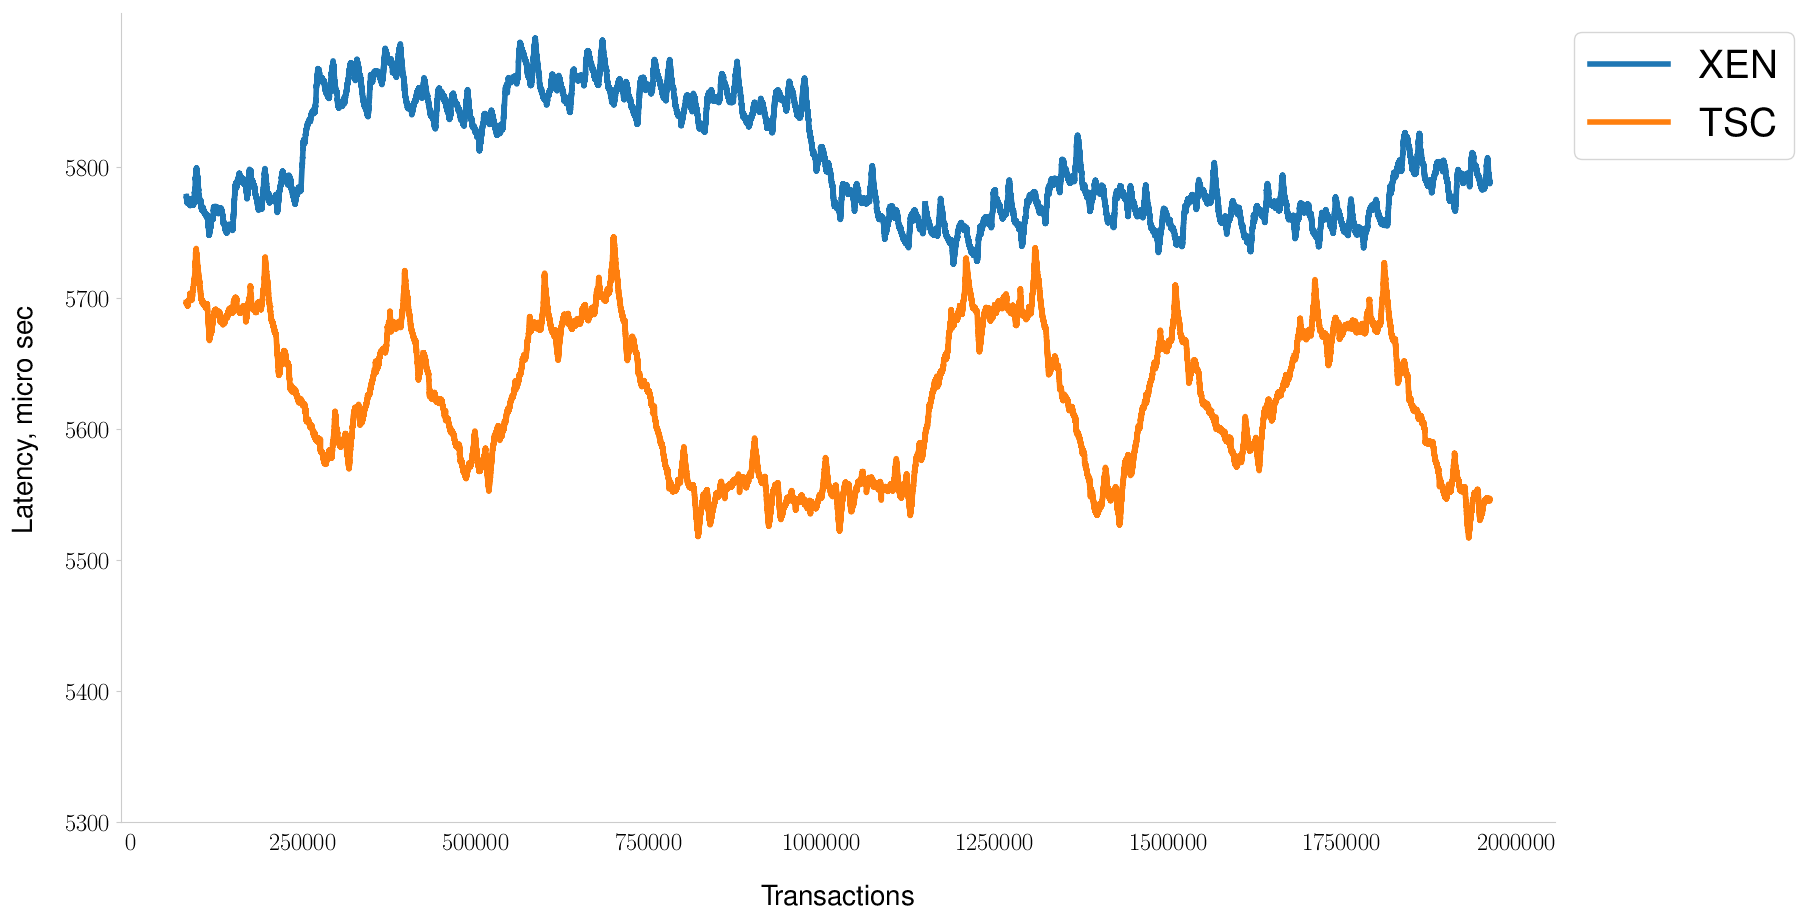
\includegraphics[width=0.9\textwidth,center]{m4_clock_source_2.png}

    \end{center}
\end{frame}

\begin{frame}
    \frametitle{}
    \begin{center}
    \textbf{Latency m5.xlarge KVM/TSC, r/w}

        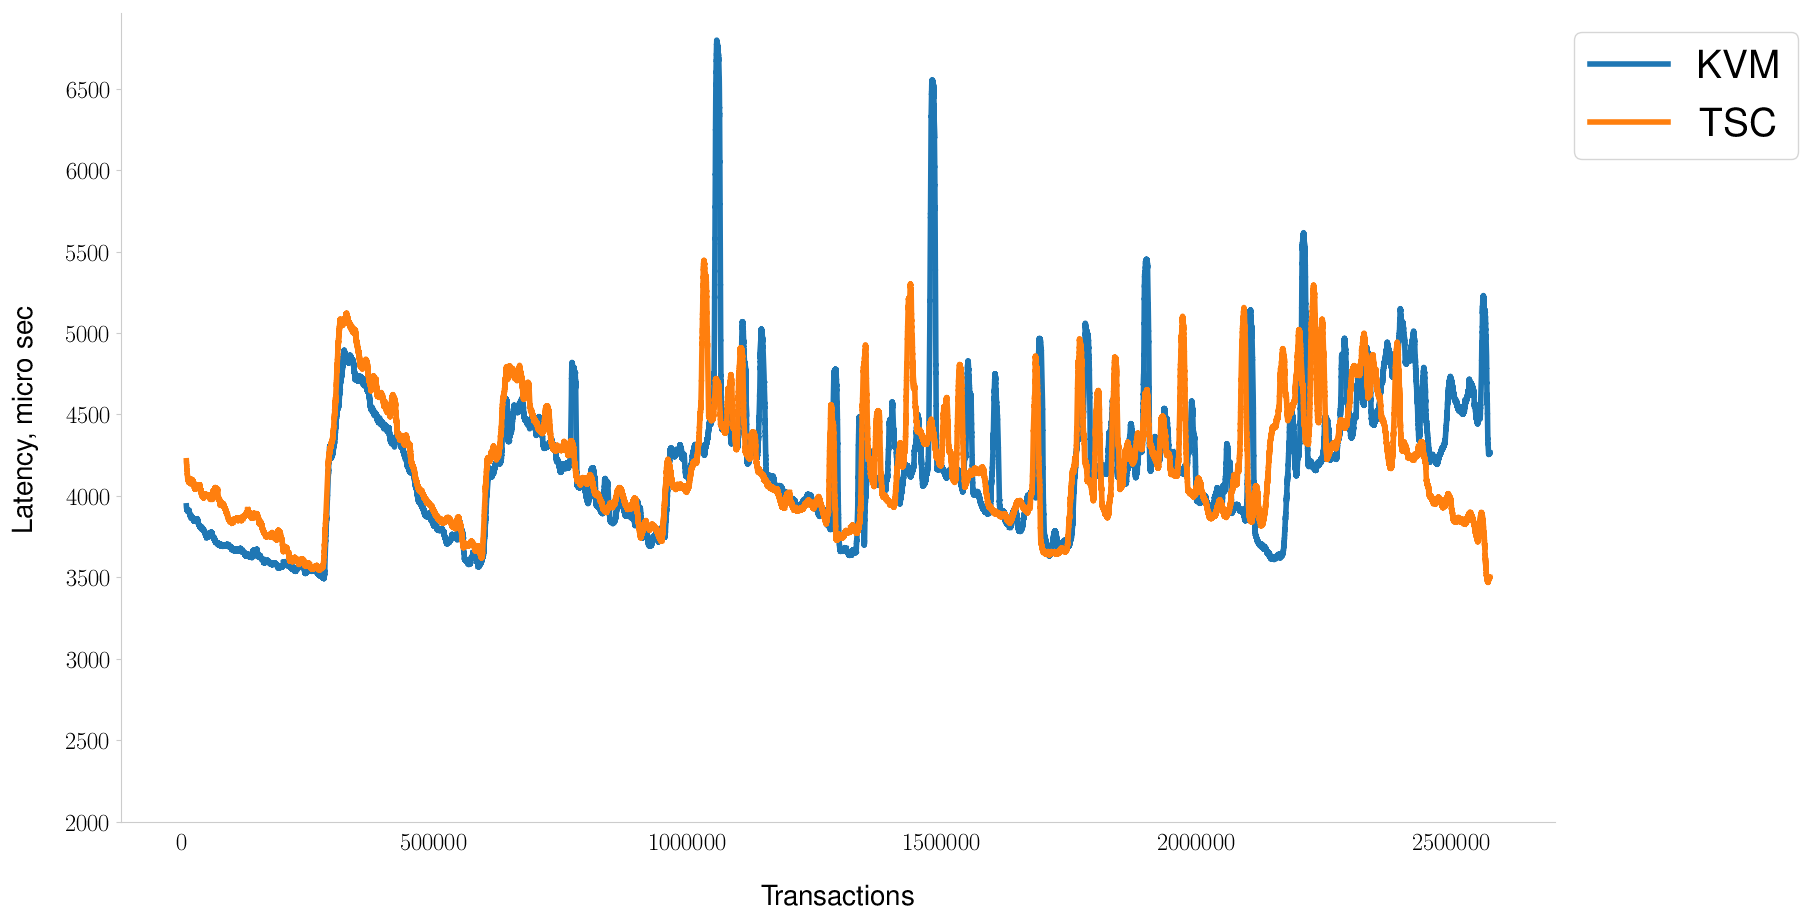
\includegraphics[width=0.9\textwidth,center]{m5_clock_source_2.png}

    \end{center}
\end{frame}

\fontsize{13pt}{14}\selectfont
\section{Containerization}
\fontsize{17pt}{18}\selectfont

\begin{frame}
    \frametitle{}
    \begin{center}
    \textbf{cgroups controllers}

    \begin{columns}
    \begin{column}{0.5\textwidth}
        \begin{itemize}[label={\MVRightarrow}]
            \item cpu,cpuacct
            \item cpuset
            \item memory
            \item devices
            \item freezer
            \item net\_cls
            \item rdma
        \end{itemize}
    \end{column}
    \begin{column}{0.5\textwidth}
        \begin{itemize}[label={\MVRightarrow}]
            \item blkio
            \item perf\_event
            \item net\_prio
            \item hugetlb
            \item pids
            \item rdma
        \end{itemize}
    \end{column}
    \end{columns}

    \end{center}
\end{frame}

\begin{frame}[fragile]{}
    \frametitle{}
    \begin{center}

        \vspace{0.3cm}
        \begin{minted}[fontsize=\normalsize]{bash}
8388   8388   postgres     blk_throtl_bio
        blk_throtl_bio+0x1        [kernel]
        dm_make_request+0x80      [kernel]
        generic_make_request+0xf6 [kernel]
        submit_bio+0x7d           [kernel]
        blkdev_issue_flush+0x68   [kernel]
        ext4_sync_file+0x310      [kernel]
        vfs_fsync_range+0x4b      [kernel]
        do_fsync+0x3d             [kernel]
        sys_fdatasync+0x13        [kernel]
        fdatasync+0x10            [libc-2.24.so]
        XLogBackgroundFlush+0x17e [postgres]
        WalWriterMain+0x1cb       [postgres]
        PostmasterMain+0xfea      [postgres]
        \end{minted}

    \end{center}
\end{frame}

\begin{frame}
    \frametitle{}
    \begin{center}
    \textbf{bklio controller}

        \begin{itemize}[label={\MVRightarrow}]
            \item CFQ \& throttling policy (generic block layer)
            \item No weight related options will work without CFQ
            \item Advisable io scheduler for SSD is noop/none
            \item Block layer do sampling to enforce throttling
        \end{itemize}

    \end{center}
\end{frame}

\begin{frame}
    \frametitle{}
    \begin{center}
    \textbf{throttle\_sample\_time}

		\begin{flushleft}
		This is the time window that blk-throttle samples data, in millisecond.
		blk-throttle makes decision based on the samplings. Lower time means cgroups
		have more smooth throughput, but higher CPU overhead. This exists only when
		CONFIG\_BLK\_DEV\_THROTTLING\_LOW is enabled.
		\end{flushleft}

    \end{center}
\end{frame}

\begin{frame}
    \frametitle{}
    \begin{center}
    \textbf{blkio}

		\begin{flushleft}
		On traditional cgroup hierarchies, relationships between different controllers
		cannot be established making it impossible for writeback to operate accounting
		for cgroup resource restrictions and all writeback IOs are attributed to the
		root cgroup.

        \normalsize{\href{
            https://git.kernel.org/pub/scm/linux/kernel/git/torvalds/linux.git/commit/?h=v4.14-rc4&id=3e1534cf4a2a8278e811e7c84a79da1a02347b8b
        }{https://git.kernel.org/pub/scm/linux/kernel/git/torvalds/linux.git}}
		\end{flushleft}

    \end{center}
\end{frame}

%\begin{frame}
    %\frametitle{}
    %\begin{center}
    %\textbf{CONFIG\_MEMCG\_KMEM}

        %\begin{itemize}[label={\MVRightarrow}]
            %\item Enabled in modern versions
            %\item PostgreSQL requires contiguous memory \\ for shared buffers
            %\item It's being allocated using slab
            %\item memory.kmem.limit\_in\_bytes is too high
        %\end{itemize}

    %\end{center}
%\end{frame}

\begin{frame}
    \frametitle{}
    \begin{center}
    \textbf{Bad neighbour}

        \begin{itemize}[label={\MVRightarrow}]
            \item memory fragmentation
            \item buddy allocator can fail \\ to find a page of proper size
            \item kernel will start a compaction process
        \end{itemize}

    \end{center}
\end{frame}
\note{
    mention explicitely "bad neighbor",
    don't forget to say that compaction can be cpu consuming
    if there is a lot of memory
}

%\begin{frame}[fragile]{}
    %\frametitle{}
    %\begin{center}

        %\begin{minted}[fontsize=\normalsize]{bash}
%# Host, normal
 %Zone: Normal
 %Free KiB in zone: 807232.00
    %Fragment size        Free fragments
    %4096                 29612
    %8192                 23308
    %16384                13495

%# Host with a container
 %Zone: Normal
 %Free KiB in zone: 109700.00
    %Fragment size        Free fragments
    %4096                 3405
    %8192                 7082
    %16384                1954
        %\end{minted}

    %\end{center}
%\end{frame}

\begin{frame}
    \frametitle{}
    \begin{center}
    \textbf{Bad neighbour}

        \begin{itemize}[label={\MVRightarrow}]
            \item PGSemaphore* funcions make use of futex
            \item Per-cpu hash table for futex with hash buckets
        \end{itemize}
    \end{center}
\end{frame}
\note{
    futex is used in PGSemaphore* functions, and make use of a hash table (per
    cpu) with hash buckets, which is a priority linked list, protected by
    spinlock. If there are a lot of futex\_key's it can cause a lot of
    collisions, and each add/remove from hash bucket cause contention on this
    spin lock.
}

\begin{frame}
    \frametitle{}
    \begin{center}
    \textbf{Bad neighbour}

        \begin{itemize}[label={\MVRightarrow}]
            \item WAL segment/heap file creation
            \item inode lock contention
        \end{itemize}

    \normalsize{\href{
        https://www.usenix.org/system/files/conference/atc16/atc16_paper-min.pdf
    }{Understanding Manycore Scalability of File Systems}}
    \end{center}
\end{frame}
\note{
    futex is used in PGSemaphore* functions, and make use of a hash table (per
    cpu) with hash buckets, which is a priority linked list, protected by
    spinlock. If there are a lot of futex\_key's it can cause a lot of
    collisions, and each add/remove from hash bucket cause contention on this
    spin lock.
}

\fontsize{18pt}{18}\selectfont
\begin{frame}
  \vspace*{2.5cm}
  \begin{minipage}[b][\paperheight]{\textwidth}
  \begin{center}

      %\raggedright%
      \linespread{1.0}%
      \usebeamerfont{title}%
      \usebeamercolor[fg]{title}%
      \if@noSmallCapitals%
        Questions?
      \else%
        \scshape{\color{black} Questions?}%
      \fi%
      \vspace*{0.3em}

      \usebeamerfont{subtitle}%
      \fontsize{13pt}{14}\selectfont
      \usebeamercolor[fg]{subtitle}%
        \begin{itemize}[label={}]
            \item {\color{black} \github\ \href{github.com/erthalion}
                                               {\color{black}github.com/erthalion}}
            \item {\color{black} \github\ \href{github.com/erthalion/ansible-ycsb}
                                               {\color{black}github.com/erthalion/ansible-ycsb}}
            \item {\color{black} \twitter\ @erthalion}
            \item {\color{black} \email\ dmitrii.dolgov at zalando dot de}
            \item {\color{black} \email\ 9erthalion6 at gmail dot com}
        \end{itemize}
      \vspace*{2.5em}%

    \vfill
    \vspace*{2em}
  \end{center}
  \end{minipage}

\end{frame}

\end{document}
